\chapter{Tyranid Transportation}

\begin{wrapfigure}{O}{\figwidth}
	\begin{center}
		
\includegraphics[width=\figwidth]{pics/15/1.png}
	\end{center}
\end{wrapfigure}
The Occurrence Border took its time leaving the system, a whole day of it in fact. 
There were three reasons for our lack of speed. 
Firstly, the tech-priests Jim had duped were seriously hindering any pursuit. 
Secondly, our bloody escape from the Station and the news that we'd been the source of the "psychic attack" had really discouraged the few small independently-owned ships that didn't rely on the Mechanicus to keep running. 
Finally, the locals' priorities had shifted drastically after a virulent fungal infection had started spreading through the Station, driving men insane with visions and melting through just about anything.

We actually felt a little bad about the whole Warp Fungus thing, but it really wasn't our fault, and it seemed like they managed to get it contained before the stuff ate more than an eighth of the Station. 
Anyway, Hannah had been looking into the stuff after the Marines had stumbled into it, and was pretty sure that it would die off, or at least lose its hallucinatory properties, without frequent exposure to the warp. 
So it would all probably work out in the end, and in the short term it bought us a little more time to prepare for the upcoming weeks of warp travel.

The last of our preparations were finished an hour before we were scheduled to re-enter the warp, and at Sarge's insistence we all wandered down to our Gellar-field adjacent quarters for a pre/post/whatever-mission briefing.

\begin{wrapfigure}{O}{\figwidth}
	\begin{center}
		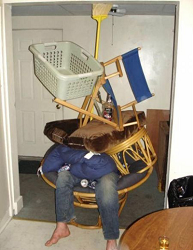
\includegraphics[width=\figwidth]{pics/15/2.png}
	\end{center}
\end{wrapfigure}
Tink and Aimy were off on one side, enjoying their usual pastime of antagonizing each other. 
The subject this time was the Tau vids Tink had acquired, specifically the ones that'd been based on our exploits on the buffer worlds, and were supposedly earning us all sorts of royalties. 
Aimy was loudly explaining that they were stupid, heretical, and concrete proof of Tink's perversion. 
Tink was holding that all of this was untrue, and that Aimy was just jealous that she hadn't been included in the vids on account of being stuck on an island with a crazy Magos at the time.

Doc was slumped over the table in the middle of the room. 
The medic had been on duty for nearly twenty hours before he'd been concussed and half crushed, and when he'd gotten back to the ship he hadn't been allowed to take a break. 
He wound up spending ANOTHER twenty hours hopped up on stimms, helping get Gravis stowed away and treating all the armsen who'd been injured during the defense of the ship. 
Doc was completely out of it, and Nubby had taken the opportunity to draw some comical facial hair on him. 
The little trooper was augmenting his doodles with a pyramid of furniture balanced on and around Doc, and was gleefully egging Tink and Aimy on.

Twitch had taped up what he claimed was the only accurate map of the Occurrence Border's tainted sections along one wall. 
I say claimed, because none of us could read the damned thing, and looking at it for any length of time made our heads hurt. 
Twitch was alternately sticking pins in the map, and talking to a servo-skull with a detpack strapped to it. 
Supposedly the Cogitator Adept was watching the skull's vid feed and answering Twitch's question via combead, but none of us could really be sure.

Finally, Fumbles was sitting in a corner of the room, grimacing at a small Tau drone with a block of white material strapped to it. 
Fio was sitting on the far side of what was definitely a blast shield, excitedly taking notes.

\begin{wrapfigure}{O}{\figwidth}
	\begin{center}
		
\includegraphics[width=\figwidth]{pics/15/3.png}
	\end{center}
\end{wrapfigure}
None of us really paid much attention to Sarge when he finally arrived, since Aimy was chasing Tink around the furniture pile by that point, but that changed when Sarge dropped the large crate he was carrying with a hollow sounding boom. 
Nubby, recognizing the crate, sidled away an appreciable fraction of the speed of light, and Fumbles, who could TASTE the rage boiling off Sarge, rather-more-literally vanished from sight. 
Before either of them could make their escape, Sarge barked an order at Twitch, who pressed a big red button on the wall marked "PANIC". 


As the exits sealed and a few dozen proximity mines activated, the foul smelling blur that was Nubby changed direction, and vanished through the only door left, which led to the bathroom. 
He locked the door behind him. 
Sarge ignored the bathroom door and the hard-to-look-at corner where Fumbles was whispering at Fio to shut up about "amazing readings" and hold still. 
He turned his attention on rest of us, and with a horrible fixed grin, asked for a status report. 


Twitch and Aimy hesitantly reported that about half of the boarders trapped in the tainted areas had been killed, captured, or found dead. 
The rest had either holed up in areas too dangerous to pursue, disappeared into the rat's nest of corridors, or just outright vanished. 
Patrols and traps had been set to contain the daemonic-feeding frenzy that would occur in those areas when we entered the Warp. 
Tink followed this up with a report on the generally-good condition of the Cells after the overhaul, and confirmation that everything was ready for entering the Warp. 
Finally, Doc was poked with a stick until he regained enough consciousness to confirm that Gravis was still alive, and that the looted medical supplies would be enough to keep him that way for a few weeks.

\begin{wrapfigure}{O}{\figwidth}
	\begin{center}
		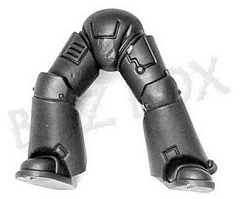
\includegraphics[width=\figwidth]{pics/15/4.png}
	\end{center}
\end{wrapfigure}
Sarge digested the three reports for a few seconds, and then poked Doc awake again. 
In an almost gentle voice, he asked the medic if he knew how Gravis' other half was doing, because Sister Valerie said she couldn't find the freezer-crate with the Space Marine's legs anywhere. 
Doc's tired brain kicked into overdrive, and dredged up an image of a dented and bullet-pocked crate being pulled off of him and tossed to the side. 
He swore, attempted to leap to his feet, and was buried as the pile of chairs around him collapsed. 
Tink, exhibiting all the tact and self-preservation instinct of a socially-retarded lemming, burst into laughter.

Sarge's attention immediately shifted to Tink. 
He opened the crate he'd carried in, took out the manifest taped to its lid, and skipped down to the section labeled Miscellaneous. 
His false grin completely gone, Sarge asked Tink if he knew where 1x Dataslate (Fecundia-pattern), 1x Astartes Grav Chute and Grapnel Harness, 2x Single-Shot Grav-Flares, and 1x Mark VII Power Armor Helmet could be found. 
Tink's poker face lasted until the helmet was mentioned and he involuntarily glanced towards where Spot was sitting. 
He looked back to find that Sarge had somehow teleported across the room and was now practically nose-to-nose with him. 
Then the shouting started.

\begin{wrapfigure}{O}{\figwidth}
	\begin{center}
		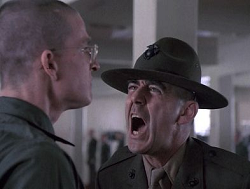
\includegraphics[width=\figwidth]{pics/15/5.png}
	\end{center}
\end{wrapfigure}
Of course, despite all the shouting and the part where he dragged Nubby out of the bathroom and held him in the air by one leg, Sarge wasn't really that angry. 
Even though he'd grown rather stodgy since his promotion, he was still a guardsman, and knew all about the importance of recycling. 
The truth was that after how badly our resupply mission had gone, he just needed to shout at someone, and the way we'd scavenged, disassembled, sold, or just-plain-lost a Space Marine's worth of wargear and legs was as good an excuse as any. 


We put up with Sarge's stress-relieving tantrum, and thanked the Emperor that he hadn't found out about what the Powersword had actually been traded for. 
I mean, Fio claimed that the chunk of wraithbone was extremely valuable and the key to all sorts of psychic engineering, but he didn't actually have any idea how it worked or what he was going to do with it… Sarge finding out that we'd lost the Powersword because our captive xenos wanted to commit some science on a spooky rock would've resulted in some REAL shouting.

So once Sarge had started feeling better, and had mandated that Sister Valerie was now in charge of Gravis' bolter and what was left of his helmet, he brought the rest of us up to date on what he, the Adepts, and the Captain had decided. 
The gist of it was that we hadn't appropriated enough fuel to reach the system where Oak's lab was, so we were going to make another stop and would offload Gravis, send a message to Oak, and repair whatever damage the Zoanthrope had caused by that point while we were at it. 
Our response to this news was conflicted at best: 
we knew that we'd be wanting another pit-stop by that point, but we really didn't want to go through all that shit again, and since the Astropaths were telling everyone that we were Inquisition-impersonation heretics, it seemed inevitable. 
Sarge assured us that he, or at least the smarter people who worked for him, had figured out a solution though.

\begin{wrapfigure}{O}{\figwidth}
	\begin{center}
		
\includegraphics[width=\figwidth]{pics/15/6.png}
	\end{center}
\end{wrapfigure}
The theory was that the Astropaths' lies would catch the attention of the Inquisition pretty quickly, and they'd send out a team to investigate what had happened on the Station. 
Unless Paths managed to purge all records of our visit, which would probably require killing pretty much everyone in the Administratum from the Prefect on down, it'd be relatively easy for the Inquisition to identify us based on vid records of Sarge and our ship, and determine that the Astropaths were full of shit. 
Then, after a judicious amount of purging, they'd send out a follow-up sector-wide message to clear our names.

The nearest Inquisition outpost was five days away from the Station; 
so call it a week to hear about the problem and travel to the Station, another week to sort things out and send the all-clear, and a third week just to be safe. 
The Captain had mapped a route that wouldn't be too far off course, and would take us to a nice, developed Imperial system with an Inquisitorial outpost of its own (just in case) in about three weeks. 
We'd dewarp REALLY far out, so if the Zoanthrope did it's head-explodey thing again it probably wouldn't kill anyone, and then discretely venture into comm range of the planet to make sure everything was okay before attempting to dock.

It was a nice, sensible plan, and all we had to do was keep the Zoanthrope contained and Gravis alive for three weeks of warp travel. 
Everyone, except Twitch, accepted that it was the best option available, and we all went off to make our last preparations. 
Two hours later the Gellar field kicked into gear, the Warp Drive tore a bloody hole in the fabric of reality, and what we fervently hoped was our second-to-last warp journey with our stupid psychic bug began. 


All-in-all, taking everything into account, and relatively speaking, the trip went well. 


Y'know by Occurrence Border standards. 


Especially if you ignore all that ominous stuff with the ghost-tyranids.


\begin{wrapfigure}{O}{\figwidth}
	\begin{center}
		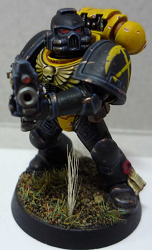
\includegraphics[width=\figwidth]{pics/15/7.png}
	\end{center}
\end{wrapfigure}
Doc, per usual, spent most of the trip in the medbay looking after Sergeant Gravis. 
The bisected Space Marine's condition wasn't good: 
the Tyranid bio-weapon that had been introduced into his system was unquestionably alive, and was constantly attacking what remained of his organs with a wide variety of poisons. 
Gravis' Space Marine biology was fighting back, but was seriously hindered by the gross trauma he'd suffered, not to mention the loss of those organs in his lower torso. 
The only thing keeping Gravis alive was his Power Armor's Automated Medicae System, a large pile of life-support machinery, and regular aid from Doc and Sister Valerie.

Since he didn't have an entire medbay to run, Doc handled Gravis most of the time. 
Sister Valerie covered for him when he was occasionally needed elsewhere for more combat-oriented medical duties, and after a week of increasing grumpiness on both their parts, her senior subordinate was put in charge of the night shift. 
Anyway, between Doc's steadily increasing experience treating the torso-fied Space Marine, and the large amount of medical supplies we'd "requisitioned" from the Waystation Alumentum Primaris, Gravis was kept, if not stable, at least only gently teetering on the brink of death. 
Initially that is.

While Doc babysat Gravis, Sarge evaluated his performance during the supply run. 
He was reasonably happy with the way things had gone after everything had fallen apart, but it seemed to him that a real Interrogator would've been able to keep things from spiraling out of control in the first place. 
He eventually came to the uncomfortable conclusion that his current social skills were rather lacking, and since the Emperor, or at least his holy Inquisition, had dumped him into a role which required them, he was going to have to fix that.

With an incredible amount of reluctance, Sarge visited the Diplomacy Adept's quarters, and asked for a few lessons on the arcane art of talking to people without shouting.

\begin{wrapfigure}{O}{\figwidth}
	\begin{center}
		
\includegraphics[width=\figwidth]{pics/15/8.png}
	\end{center}
\end{wrapfigure}
The Diplomacy Adept found teaching Sarge to be rather difficult, mostly because our fearless leader was so set in his ways. 
In Sarge's book Deception and Disguise were accomplished using stuff like helmets on sticks, camo paint, and smoke grenades; 
Inquiry and Intimidation shared a definition, and involved little, if any, talking on his part; 
and the pages that covered Blather and Charm had been removed to make more space for the chapter that covered Command. 
Regardless of the difficulty involved in reversing a lifetime's worth of sergeanty preconceptions though, the two of them did make some progress as we travelled. 
Admittedly it was very slow progress, and involved an awful lot of yelling, but progress none-the-less.

For their part, Tink and his fellow xeno-culturists made some progress of their own during the voyage. 
The wonder-team of Fio, Jim, and Tink were in charge of Zoanthrope Containment, with occasional assistance from the Xenologist Adept and Hannah (if she was hiding from her problem-prone tech-acolytes in the Cells). 
They'd refurbished everything in record time before we entered the warp, and afterwards things had gone surprisingly smoothly. 


Thanks to all the parts Nubby had acquired, the Psi-Suppressors, Shielding, and Warp Shroud had all been repaired and improved to the point where they were very nearly within the minimum recommended strength for containing a Delta level psyker during warp travel, and the Stasis Field was working perfectly for a change. 
All that had to be done in the Cells was a bit of daily inspection and maintenance, which was always carried out quickly, because the Zoanthrope had acquired an unsettling presence ever since Sarge's partially-slagged shield had gotten wrapped around its head. 
It was hard to shake the feeling that, despite the stasis field, the eyes under the metal were watching you.

Of course, the reduced maintenance requirements of the cells meant the nerds were able to spend time on other things.

\begin{wrapfigure}{O}{\figwidth}
	\begin{center}
		
\includegraphics[width=\figwidth]{pics/15/9.png}
	\end{center}
\end{wrapfigure}
"Other things" in this instance translating to helping with important ship maintenance in Jim's case, and committing all sorts of tech-heresy in Tink and Fio's. 


Actually, you couldn't really call what Fio was doing tech-heresy, it was more a case of tech-heathenism, him being a xenos and all. 
He was quite fixated on the piece of Wraithbone we'd acquired, and spent every scrap of his free time tinkering with it. 
Some days he'd be wiring it into every device in the Cells, other times he had it mounted on a drone and trailing Fumbles through the ship, and occasionally he could be seen wandering around with the big white block strapped to his head like a demented hat. 
Tink said it was all very scientific, Jim and Hannah refrained from commenting, and the rest of us were just glad it kept the mouthy little xenos busy.

Tink, deprived of the helmet he was cannibalizing to upgrade Spot and perhaps motivated by a sense of shame at his inappropriate behavior (not likely), dedicated his time to a more practical project: 
the damaged Emperor's Scythes Stealth Shuttle. 
During our Zoanthrope-acquiring trip the ship's tech-acolytes had finished de-fungusing it, but after that it'd just been left to sit in a shuttle bay on account of how it was completely non-functional. 
The fungus had eaten away a lot of armor and stealth materials, and had pretty much destroyed the landing gear, but the real problem was that a bunch of spores had gotten into the shuttle's circuitry. 
Some of the best piloting, navigation, and stealth-control systems a forgeworld could make had been reduced to hunks of corroded metal and silicon. 


Jim and Hannah had declared the shuttle unfixable without the aid of a fully stocked manufactorum and access to the shuttle's blueprints. 
Tink however, saw the shuttle as both a challenge and an opportunity, and had snuck a few parts of both Imperial and Xenos origin which had nothing to do with psyker-containment onto the list he'd given Nubby.

\begin{wrapfigure}{O}{\figwidth}
	\begin{center}
		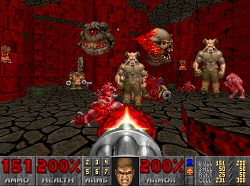
\includegraphics[width=\figwidth]{pics/15/10.png}
	\end{center}
\end{wrapfigure}
When he found about about the project, Sarge briefly considered yelling at Tink for scavenging more of the Emperor's Scythes' stuff, but decided it did technically count as repairing the shuttle, and we were already up to our eyes in xeno-tech heresy anyway. 
Also, there was a chance we'd get a working stealth shuttle out of it. 
For their part, Jim and Hannah just ignored all mention of the Shuttle, and added the its bay to the list of places their tech-acolytes weren't allowed to go. 
The rest of us didn't have any input on the subject, because we were either busy with Gravis or dealing with the increasing level of warp-activity in the Occurrence Border's tainted areas.

The initial high volume of anomalies and incursions had been expected. 
The things that usually discorporated after finding the tainted sections devoid of anything living had swarmed the trapped boarders and grown strong. 
Several varieties of warp beasts, minor daemons, reanimated corpses, and what Nubby would tell anyone who'd listen was a Bloodthirster (despite it's lack of height, axe, or wings) had tried to claw their way into the more habitable sections of the ship during the first few days of transit. 
Thanks to the fact that we'd known the general location of the boarders, the unholy horrors had come through to find numerous traps, swarms of detpack-armed suicide skulls, the hardened priests and armsmen that made up the Ship's Watch, and a few well-armed guardsmen waiting for them.

Even with prepared positions and numerical superiority though, tackling warp creatures can be tricky. 
Over the three days it took the last of the boarders to expire, the daemons and the anomalies that manifested around them took a small but significant toll on the defenders. 
Some men were torn apart, others went insane, an unlucky few ran afoul of the Occurrence Border's chronic mechanical problems, and one or two forgot to check what was on the other side of a door before stepping through it.

\begin{wrapfigure}{O}{\figwidth}
	\begin{center}
		
\includegraphics[width=\figwidth]{pics/15/11.png}
	\end{center}
\end{wrapfigure}
Of course none of US were on the casualty list. 
Prior experience with this sort of thing, not to mention better quality weapons and a rather pragmatic approach to questions like "Do you think that thing with the tentacles is still in there?" meant that we made it through without significant injury. 


Insignificant injuries and close-calls are a different matter mind you. 
Something in the third wave of daemons threw Fumbles' powers out of whack and caused a few burns and bruises for everyone present. 
And then there was a hairy moment when Twitch barely stopped Aimy from stepping through a door that inexplicably opened into one of his minefields. 
After that one of Nubby's augmetic feet had to be plasma-cut off and replaced on account of how he tried to kick a nurgling in the nadgers. 
Oh, and the ONE TIME Doc came down to help with casualties, a priest he was treating tried to eat his face and had to be exorcised (see: 
clubbed into unconsciousness) using his own book of holy verse.

Anyway, things calmed down after the third day, and once the various bits and pieces had been incinerated, jettisoned, or tossed back into the tainted section, the bulkheads were resealed and everyone got back to their usual routine. 
Unfortunately things didn't STAY calmed down: 
over the next few days reports started filtering in of creatures haunting the corridors near the tainted areas. 
This wasn't unusual in and of itself, since every time the Navigator hit a bump in the warp stuff would leak through all over the ship and there had just been a daemonic incursion in the area to boot, but the witness reports were worrying: 
they matched the ones we'd received during our previous week of warp travel.

\begin{wrapfigure}{O}{\figwidth}
	\begin{center}
		
\includegraphics[width=\figwidth]{pics/15/12.png}
	\end{center}
\end{wrapfigure}
Last time Aimy, Twitch, Nubby, and Fumbles had tracked the problem down to an infestation of what had appeared to be tyranids. 
It turned out that they weren't proper nids though, since shortly after they'd been killed, the bugs' remains had started reforming in a distinctly warpy fashion, and then they'd just sort of vanished when we finally dewarped. 
We'd decided that the whole thing had just been some sort of warp phenomena caused by the psychic containment in the Cells failing, and the Zoanthrope sort of passively screwing with reality. 
This explanation was ruined by the fact that, despite the Cells being all fixed up, the warpy-nids had come back. 
Or maybe they hadn't, it was all a bit of a mess. 


The problem was that, this time, the tyranid-shaped creatures that Nubby drew out with his damsel-in-dis-dress routine were different: 
they had an appearance and behavior that could best be described as ghostlike. 
Not ghostlike as in "sneaky", but ghostlike as in "like a ghost". 
Literally. 


Now, the Occurrence Border was practically littered with warp-ghosts, but human ones. 
For the most part they just wandered around re-enacting their lives and deaths, with the occasional bout of unsettling whispering or screaming thrown in. 
They were harmless by and large (and even provided decent entertainment on slow days), but that could change if someone or something managed to get their attention and drag them into sync with what passed for reality. 


Anyway, the tyranids we found literally haunting the fringes of the tainted areas displayed all the signs of being warp ghosts, except y'know, tyranid ones. 
They sort of milled around in the shadows, drifting through walls, making clicking noises at each other, and gnawing at stuff that wasn't there, until we got too close or had Fumbles poke 'em. 
Then every ghost-nid in the area would swarm in around the agitated one, and become an awful lot more solid until a few bolts of plasma blew them into black and green smoke.

\begin{wrapfigure}{O}{\figwidth}
	\begin{center}
		
\includegraphics[width=\figwidth]{pics/15/13.png}
	\end{center}
\end{wrapfigure}
At first the ghost-tyranids were just puzzling: 
based on the little we knew about the warp and what information our xenology adept could provide, it shouldn't have been possible. 
Your average nid doesn't have a mind, much less a soul, and those are pretty much requirements for being a ghost, otherwise the warp would be littered with ghost-bricks/trees/rocks/whatever. 
Everyone agreed that something odd was going on, but no one could figure out exactly what it was. 
At first we just blamed the Zoanthrope, but Jim and Fio checked and couldn't detect any psychic energy leaking out of the Cells, and Fumbles backed them up.

Other theories were raised, such as the ghost nids being a psychic projection built upon the crew's collective unconscious fear of tyranids, or them being the result of the Hive Mind reaching across the warp to smite us, or everything being caused by the Ancient Heathen Insectoid Idol stored in Cargobay E-71/3 which had driven all who looked upon it insane. 
These were all shot down for various reasons, such as the fact that, according to 'Ol Bill, the idol's various limbs had been holding up a plasma conduits for thirteen years now without any significant problems. 
Twitch, of course, held fast to his theory that the Tyranids aboard the Hive Ship which had been sucked into the warp by the Scythe's vortex bomb had made an alliance with the daemons of chaos and an unstoppable tide of Daemonids would rampage across the galaxy. 
No one but Aimy bothered to argue with him, and in the end the rest of us decided that the ghost-tyranids were probably still somehow the Zoanthropes fault, despite all evidence to the contrary.

To return to the point though, the ghost-nids were puzzling AT FIRST. 
This wasn't because something happened which explained everything, it was because they quickly became far too serious a problem to waste time actually thinking about it.

\begin{wrapfigure}{O}{\figwidth}
	\begin{center}
		
\includegraphics[width=\figwidth]{pics/15/14.png}
	\end{center}
\end{wrapfigure}
The number of ghost-tyranid sightings quickly rose, as did the number of attacks. 
We'd tried to nip the problem in the bud, of course: 
a busy two days had been spent antagonizing ethereal hormagaunts into solidity, and then shooting them. 
Unfortunately, they didn't stay dead, even when we got the Confessor himself to come down and wave his censor around after we shot them. 
It'd take a few hours, but eventually a bug that Fumbles claimed was same one would drift back to the spot where we'd killed it, and resume its seemingly-random wandering.

An expedition into the tainted areas to see where they were coming from was proposed, but after some careful thought, we decided that we didn't actually want to die horribly in a twisted nightmare of non-euclidian geometry and bug-shaped warp monstrosities. 
We might have really considered it if the ghost-tyranids had seemed interested in launching attacks on the rest of the ship, but as far as we could tell they were content to just sort of hang out. 
Over time, the steadily increasing number of ghost-bugs would result in them wandering deeper into the ship, but otherwise they stayed put unless someone got near them. 
Lacking any viable solution, or the motivation to take a real risk to find one, the Captain agreed with our decision to just set up a killzone around the tainted areas and contain the apathetic ghost-tyranid menace.

The containment strategy wasn't sustainable in the long run, since the number of bugs was inexorably increasing, and they were able to expand in three dimensions as well as through walls too. 
But we were pretty sure that if we gave a little ground when the numbers got to high, it'd work long enough for us to reach our next resupply point. 
Also, if things got really bad, we could always dewarp and sort things out at the expense of a few days of travel time. 
So since there wasn't any immediate crisis, we settled into a slightly more stressful than usual routine, and got on with our lives.

\begin{wrapfigure}{O}{\figwidth}
	\begin{center}
		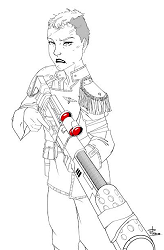
\includegraphics[width=\figwidth]{pics/15/15.png}
	\end{center}
\end{wrapfigure}
Aimy assumed command of the entire lower-aft portion of the defense. 
She didn't actually ask for permission or anything mind you, she just walked down there and started bossing everyone around. 
The only reason that the Captain and his Master-at-Arms didn't kick up a huge fuss about this blatant disrespect was that Aimy was actually very good at this sort of thing, having been born and raised for infantry command before her career change to Inquisitorial-Gooning. 
The rest of us noticed that, despite how much she complained about the poor quality of her troops compared to her old regiment, Aimy seemed far happier than she'd been since her disastrous mission with the half-mad Magos. 
Or if not happier, at least less prone to spontaneous violence.

Since Twitch, not to put too fine a point on it, wasn't really sane enough to command a squad, much less an entire flank of the defense, his assistance to the containment effort was a bit more ad hoc. 
He scampered around, shoring up defenses and setting up traps without any discernible rhyme or reason, and everyone else just had to adjust their deployments to fit. 
It was all surprisingly effective, though it retrospect it shouldn't have been, he'd spent more time patrolling the borders of tainted areas than anyone except 'Ol Bill and his senior Engineers, and knew which spots were defensible and which weren't by heart.

Initially, Nubby just sort of mooched around the various fronts "assistin wif da supply effort", but since his partner in petty crime was the only psyker around who wasn't busy steering the ship, this profitable arrangement didn't last. 
We'd quickly discovered that Fumbles' ability to sense the ghost-nids from quite far away and through walls was invaluable, especially since he could share what he sensed with anyone nearby. 
He was constantly in demand as a spotter, and Nubby was dragged along to act as backup and moral support.

\begin{wrapfigure}{O}{\figwidth}
	\begin{center}
		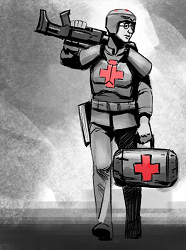
\includegraphics[width=\figwidth]{pics/15/16.png}
	\end{center}
\end{wrapfigure}
As has been mentioned, the rest of us had other things to do, and the ghost-nid situation really didn't change that. 
I mean, if you stop work every time an army of warp-spawned insectoid spirits lays siege to your ship, you'll never get anything done. 
So we all just sort of muddled along, trying to hold everything together, as the trip continued and things got progressively worse.

In the case of Doc's treatment of Sergeant Gravis, "got progressively worse" is a perfect summary. 
The Space Marine's condition went steadily downhill, and not in the ways Doc or Valerie had been prepared for. 
There were seemingly random seizures, spikes in neural activity that indicated horrible nightmares, inexplicable changes in the behavior of the bio-toxin, and even a few spontaneous mechanical failures in the life support machinery. 
It got to the point where Gravis-watching was a 24-hour, no-distractions duty, because the second he was left alone something would invariably go wrong. 
Doc, not being born yesterday, blamed all these problems on the warp in general and the Zoanthrope in particular, but he couldn't figure out the why or how, and had no idea what to do about it.

Lacking any proactive treatment ideas, aside from exiting the warp or killing the Zoanthrope, Doc dedicated increasingly large portions of his time to Gravis-watching, and developed a rather disturbing tendency to talk to the comatose Space Marine. 
Tasteless jokes about Valerie getting jealous aside, we began to worry about him, but we were getting near the end of the trip by the time things got really worrying, and he seemed to recover a bit after his theory about the Zoanthrope being the cause was confirmed.

\begin{wrapfigure}{O}{\figwidth}
	\begin{center}
		
\includegraphics[width=\figwidth]{pics/15/17.png}
	\end{center}
\end{wrapfigure}
Actually, it wasn't just Doc's theory that was proven, our suspicions about there being a link between the ghost-nids and the Zoanthrope were confirmed too. 


What happened was that, three days out from our destination, nearly a quarter of the psi-suppressors in the Cells failed at once. 
This didn't come as a complete surprise mind you: 
even in stasis, the Zoanthrope's mere psychic presence, not to mention the warp itself, wore down the machinery and shielding that restrained it. 
Tink, Fio, and Jim had been dedicating more and more of their time to inspections and maintenance, but there was only so much that they could do given the general kludged-together nature of the Cells. 
So they'd been sort of ready for something like this to happen, and had made sure that someone was always on duty. 
When the failure happened, Jim had been right there to start fixing things, and both Fio and Tink had arrived within minutes to help. 
Sarge showed up too, but he didn't actually help in any meaningful way, he just really wanted an excuse to ditch the horrible self-inflicted purgatory of his diplomacy lessons.

Anyway, during the fifteen or so minutes of reduced psi-suppression on the Zoanthrope the following happened: 

\greentext{>The spawn rate of ghost-nids drastically increased, a few higher forms started appearing, the entire swarm began acting far more in touch with reality and became significantly harder to kill.}

\greentext{>All sorts of warp phenomena occurred throughout the ship.}

\greentext{>The temperature on the main atmospheric regulator got stuck at seven degrees. (This was probably unrelated, but by then we were blaming EVERYTHING on the damned bug)}

\greentext{>Fumbles suffered some sort of combination hallucinatory and convulsive episode, and wound up clawing at his face and breaking his goggles.}

\greentext{>The Navigator sent us a very angry note about the importance of not distracting him while steering.}

\greentext{>Sergeant Gravis caught fire. Again.}


\begin{wrapfigure}{O}{\figwidth}
	\begin{center}
		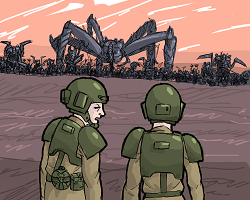
\includegraphics[width=\figwidth]{pics/15/18.png}
	\end{center}
\end{wrapfigure}
So yeah, it was a pretty unpleasant experience, especially since it was actually a minor failure compared to the some of the stuff that had broken during our last trip, and therefore raised all sorts of questions about the Zoanthrope's powers. 
Not that we had much time for pondering though, because the following three days were absolutely exhausting.

Most of the problems caused by the failure were dealt with immediately: 
The suppressors were repaired without the Zoanthrope breaking out of stasis and trying to killing everyone. 
Doc actually had a fire extinguisher ready, put Gravis out before the eldritch flames did any real damage, and handled everything else that went spontaneously wrong during the brief loss of suppression. 
Nubby managed to restrain Fumbles before he clawed out his own eyes, got the psyker to safety, and was even able to scrounge up another pair of extra-large welding goggles (which may or may not have had "Bill's DO NOT STEAL" written on them). 
Lastly, thanks to a general retreat order by Aimy and the Captain, plus Twitch's suspiciously well-placed fallback points, relatively few men died to the temporarily empowered ghost-nids. 


Unfortunately, even though the ghost-nids lost focus and weakened again after the psi-suppressors were back online, the increase in their numbers was permanent. 
Containment became significantly more difficult, especially since, in some places, the defense had been pushed back to rooms that Ol' Bill said were important to the running of the ship. 
It wasn't a good situation, but then again, it could've been worse: 
both ammo and food were plentiful, it wasn't snowing or raining aside from the occasional drizzle of supernatural blood, and there weren't any Commissars. 
On the Official Imperial Guard Scale of Horrible Meatgrinder Defenses it was only about a 3. 
Of course, anything that even shows up on that scale isn't something you want to deal with while travelling through the warp...

\begin{wrapfigure}{O}{\figwidth}
	\begin{center}
		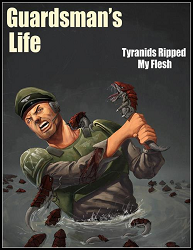
\includegraphics[width=\figwidth]{pics/15/19.png}
	\end{center}
\end{wrapfigure}
The question of whether to just dewarp in the middle of space and try to sort everything out was raised again, but since we were so close to our destination, Sarge and the Captain decided we could tough it out. 
The rest of us reluctantly agreed, and put everything we could into holding out three more days.

Reinforcements were mustered from the crew, those wounded who could still fight were put back on the line (including a rather shaken Fumbles), and our fearless leader oh-so-regretfully abandoned the last of his diplomacy classes to personally take over the nastiest piece of the line. 
Finally, Tink and Fio were told that, regardless of how creepy being around the Zoanthrope was and how important they felt their pet projects were, they now LIVED in the Cells, and horrible things would happen to their vids if another mechanical failure occurred. 


It was a hectic, terrifying, and heroism-filled three days, which really reminded all of us of our time in the Guard, though with less indiscriminate shelling and a rather inferior brand of trench-mates. 
Not that the armsmen of the Occurrence Border weren't good fighters, they just… weren't Guardsmen. 
Anyway, complaints about troop quality aside, we managed to hold out without any more complete disasters. 


There were a few tense moments, such as when Tink got as far as reporting that a cascading suppression failure was imminent before he figured out how to use his plasma gun as a backup battery. 
We would've congratulated him on his ingenuity, but it took him about half an hour to remember to tell us that things had been stabilized and we weren't about to die. 
Another bad spot was when Sarge finally abandoned the forward power management, water purification, and toothpaste distribution room, only to have something break in it five minutes after he left. 
It took a three-hour counter offensive, spearheaded by all of us except Aimy, to get Ol' Bill up there to fix the thingy that'd gotten stuck in the whatsit.

\begin{wrapfigure}{O}{\figwidth}
	\begin{center}
		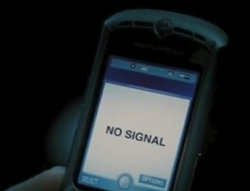
\includegraphics[width=\figwidth]{pics/15/20.png}
	\end{center}
\end{wrapfigure}
In the end though, we made it. 
A few hours before our original scheduled dewarp time, but not a second too soon, we arrived at that bastion of Imperial civilization widely known as: 
"That system with two planets and an Inquisition base that's pretty much on the way. 
No not that one, the one with the BLUE star." 

As the Occurrence Border left the warp, the massive swarm of ghostly tyranids just faded away. 
It was actually sort of awkward for those of us on the line, and sheer paranoia kept everyone at their posts for nearly an hour before victory was declared and we all went off to get some sleep. 
The only people left awake were those who'd been augmented past the need for the pathetic meatbag concept of sleep, and the poor bastards in charge. 
Sarge hiked his way up to the bridge to verify that we were in the correct system and that no stellar disasters, xenos invasions, or heretical uprisings were occurring in it, and to send a message to the Inquisition base. 
Unfortunately, that last part proved unexpectedly difficult.

Due to our recent problem with head-exploding waves of psychic energy, we came out of warp way out on the edge of the system. 
Of course the universe despises all rational planning, so the Zoanthrope stayed completely quiet during the transition, and all our careful precaution accomplished nothing aside from leaving us several days of normal space travel away from our destination. 
In fact we were so far out that our sensors could barely even pick out the largest ships and stations around the planets, and it'd be days before we got into vox range. 
This annoyed Sarge, who wanted to get started on the whole process of proving our identity and requesting aid so he could stop worrying. 


The Captain sympathized with him, and rather sarcastically asked Sarge if he wanted to try to make a micro-warp to get closer to the planets. 
Sarge told him to go fornicate with a waterfowl, and then wandered off to try and nap away his paranoia.

\begin{wrapfigure}{O}{\figwidth}
	\begin{center}
		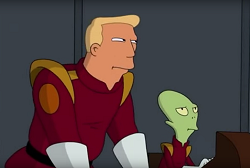
\includegraphics[width=\figwidth]{pics/15/21.png}
	\end{center}
\end{wrapfigure}
The rest of us weren't too concerned about the travel time, since moving through normal space was downright relaxing by our standards. 
If left to our own devices we probably would've spent the entire time asleep, drunk, or watching heretical cartoons, but Sarge didn't approve of idle troops. 
After a mere sixteen hours of sleep, he dumped every one of us out of our nice-warm bunks, gathered the entire team plus Ol' Bill and Jim together, and began giving orders.

The impromptu briefing started with Sarge informing us that the Captain had spotted three ships of indeterminate size heading our way, and per tradition, Twitch interrupted to tell everyone that he HAD A BAD FEELING ABOUT THIS. 
After a few minutes had been wasted on half-comedic speculation, Sarge shared the Captain's assurance that this was a perfectly normal response to how far out we'd warped in. 
He claimed that it was, in fact, a good thing, since they'd be able to help us by passing our vox messages on to the Inquisition base earlier than we'd expected. 
It'd still be over a day before we were in range though, and in the meantime, there were things to do.

Tink and Fio were told that their pet-projects were still on hold until they made sure every system in the Cells was working fine and compiled yet another parts list. 
Doc, who was annoying chipper after his first real break from Gravis-watching in over a week, was told to ditch the Marine on his girlfriend and get his gear ready. 
The Adepts were told to whatever adepty things needed doing before we talked to whoever ran the local Inquisition base, except for the Cogitator Adept, who was ordered to use his data-thingys and compu-whatsits to figure out where the ghost-nids had been coming from. 
He responded with a lot of useless technobabble and complaints about not being a demonologist damnit, but after Sarge glared at him for a while he went off to his closet and got to work. 
Everyone else was ordered to get ready for a short expedition.

\begin{wrapfigure}{O}{\figwidth}
	\begin{center}
		
\includegraphics[width=\figwidth]{pics/15/22.png}
	\end{center}
\end{wrapfigure}
A few hours later, the Cogitator Adept delivered a dataslate containing what Twitch and Ol' Bill assured us was a map marking four locations in the Occurrence Border's various tainted areas. 
The rest of us took their words for it, and Twitch was put in charge of deciphering it into three-dimensional directions. 
Sarge chose the location in the lower-aft tainted section as our first target, on account of how it was near the other thing he wanted to sort out with the expedition, and we set out with Ol' Bill and his gaggle of Engineers and tech-acolytes in tow.

Now, we called it an expedition, and went in heavily armed, but outside of the Warp the tainted areas weren't THAT dangerous. 
Yes, they were still contaminated with warp energy which manifested as all sorts of phenomena, but they were generally minor things, like whispers, winds, flashes of movement, and the non-insectoid variety of ghost. 
The krootoids and other vermin which wandered into the area and wound up horribly mutated, and occasionally possessed, were only a minor inconvenience, and warp-entities which can survive in normal space without some kind of host are rare. 
Really, it was just a matter of carefully avoiding mechanical hazards and the occasional persistent anomaly, such as the time loop on on sub-deck U-3, the room stuck at five degrees kelvin, the time loop on sub-deck U-3, the perpetually bouncing ball, and the time loop on sub-deck U-3. 


We reached the area that the Cogitator Adept had calculated as the center of the ghost-nid infestation without any incidents more serious than a tech-acolyte getting slightly electrocuted and Nubby getting stuck during an attempt to bypass a leaking plasma conduit via air shaft. 
Unfortunately, when we got there we didn't find any daemonic portals, eldritch devices, Tyranid hives, or anything else we could cover with detpacks.

\begin{wrapfigure}{O}{\figwidth}
	\begin{center}
		
\includegraphics[width=\figwidth]{pics/15/23.png}
	\end{center}
\end{wrapfigure}
All we found at the geographic center of the ghost-nid infestation was a few empty rooms and corridors. 
We had Fumbles take a look around just in case, but while he claimed the area were slightly more tainted it's surrounds, it seemed to him like it was just the side-effect of being filled with ghost-nids for longer. 
We debated exploding the entire area, just on the off chance it would accomplish something, but Ol' Bill asked us not to. 
So, lacking anything productive to do, we headed down to Cargobay E-71/3, home of a few dozen plasma conduits and an Insanity-Inducing Ancient Heathen Insectoid Idol that had been repurposed as an architectural support.

Operating on the theory that, even if it wasn't related to our bug problem, it probably wasn't good to have a giant eldritch statue just sitting around in a warp-tainted cargobay, we asked Ol' Bill to figure out a way to disentangle the plasma conduits from the Idol. 
Not so we could study it of course, that would be silly, we just wanted to make sure that the engines wouldn't explode or something when we destroyed the thing. 
Ol' Bill grumbled a bit about not fixing what isn't broken, but he and his boys threw a tarp over the thing's horrible mind-shattering visage, and began scavenging replacement parts from the surrounding area.

A few hours later the various plasma conduits, pipes, and wires were being supported by a haphazard network of metal bands, clamps, crates of expired food, and three of the room's grav-plates fastened to the ceiling. 
The tarp-covered Idol was dragged to the center of the room, and a pair of melta-bombs with what looked suspiciously like crossed-scythe insignias on their sides were fastened to it. 
The horrible chittering screaming went on for quite a while, but it trailed away as we reached the edge of the tainted area, and nothing else really happened. 
Well, aside from a 11% drop in the efficiency of Engine 6, and half of the aft sensors overloading. 
Ol' Bill said he told us so.

\begin{wrapfigure}{O}{\figwidth}
	\begin{center}
		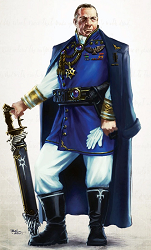
\includegraphics[width=\figwidth]{pics/15/24.png}
	\end{center}
\end{wrapfigure}
By the time we got back from our expedition the distance between us and the three approaching ships had closed to the bare edge of our vox system's broadcast range. 
Now that they were closer, our sensors had identified the ships as a Navy frigate and a pair of smaller SDF ships, so Sarge, the Captain, and the Adepts decided not to mess around with subtlety, and announce our identity and intentions off the bat.

Remembering his recent lessons on the importance of stance, dress, and overall first impressions, Sarge scrounged together a replacement for the Inquisitorial costume and evil goon uniform which had been rather gleefully abandoned in men's room garbage bin. 
After he'd more or less ripped Doc's evil goon uniform in half during his attempt to make it fit, he settled for wearing one of the Captain's spare uniforms and hung his Interrogator's Rosette in clear view. 
Suitably outfitted, Sarge then spent nearly two hours with the old Diplomacy Adept, recording a two-minute vid which primarily consisted of his name and rank, a request that his message be forwarded to the local Inquisition base, and the digital authorization code from his rosette. 
This arduous task completed he joined the rest of us for a few games of cards while the message crawled across the system at the annoyingly-slow speed of light.

Four hours and several thrones lost to Nubby and Fumbles later, it occurred to us that we really should've gotten a response by then, and we all trooped up to the bridge to see if something interesting was happening. 
We arrived just in time to hear one of the sensor techs report that all three approaching ships had increased their acceleration, and four more had left orbit. 
Twitch informed everyone that he had a REALLY bad feeling about this.

\begin{wrapfigure}{O}{\figwidth}
	\begin{center}
		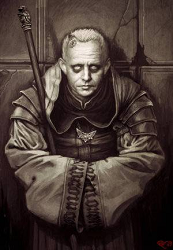
\includegraphics[width=\figwidth]{pics/15/25.png}
	\end{center}
\end{wrapfigure}
Over the next few hours the vid was re-sent multiple times, a request for confirmation of receipt was added, an audio-only version was sent, and some tech-acolytes were sent out in a shuttle to check that our vox system was actually sending and receiving correctly. 
All this effort accomplished absolutely jack shit aside from increasing the acceleration of the approaching ships even further, and raising the local paranoia level to amazing heights.

An emergency meeting of everyone who could contribute to a serious conversation on our options was called, and the rest of us invited ourselves along anyway. 
There was some initial complaining by Jim, the Adepts, and other such stuffy people about how the whole meeting was pointless, since no one actually knew anything useful about the situation, so all that anyone could do was make wild guesses based on hearsay and unsupported speculation. 
That sounded fine to us, because it was how we made most of our decisions, and everything typically worked out, so we ignored their whining.

The initial topic of conversation was just what in the Emperor's name was going on, and if there was any chance we could sort it out. 
All theories stating that the approaching ships were friendly, and there was just some sort of inexplicable reason why they just couldn't talk to us, were immediately thrown out on the grounds that the universe didn't work that way.Twitch's theory that the local naval forces had been taken over by an advance force of Daemonids, or possibly Kommados, was dismissed for similar reasons. 
The general consensus we arrived at was that the locals were following the Astropathic kill-order that had been sent out by the insane Choir-Master, which had probably included something like "Disregard any messages they send, especially ones containing Inquisitorial Authorizations Codes". 
This raised a bunch of new questions though, the primary one being: 
why the hell hadn't the Inquisition rescinded that order yet.

\begin{wrapfigure}{O}{\figwidth}
	\begin{center}
		
\includegraphics[width=\figwidth]{pics/15/26.png}
	\end{center}
\end{wrapfigure}
Since it was unimaginable that the Inquisition hadn't noticed a sector-wide astropathic message to kill someone, much less a whole ship of people who were in their records as Inquisitorial agents, we felt sure that an investigation into the incident on the Station had at least been started. 
There was of course the remote possibility that whoever they'd sent to investigate had completely botched things and either swallowed the Choir-Master's obvious lies or been offed by the locals, but that seemed unlikely. 
Despite our personal experiences, the Inquisition on the whole is rather notorious for its incredulity and competence.

Doc suggested that the investigator's ship could've been lost in the warp, or that other warp-travel related shenanigans had occurred, such as our own warp-journey taking only a few hours of real time as opposed to the three weeks we'd experience. 
The Captain shot down that last explanation, claiming to be absolutely certain for some technical reason that three and a half weeks of real time had passed, but allowed that Doc had a point about the dangers of warp-travel delaying the investigation. 
The Diplomacy Adept also raised a valid point, which was that, given the time it would take to investigate the Station and our direct route, no Inquisitorial couriers would've reached the system before us. 
This meant that any "No, these Astropath-exploding people are not heretics, don't kill them" order from the Inquisition would've been sent out via Astropath, so there was a very real possibility that a few things got… lost in translation, for instance the No, Not, and Don't.

Both of those explanations sounded good enough for us, but they didn't account for why the local Inquisition base wasn't doing anything, and that was a more pressing concern at present.

\begin{wrapfigure}{O}{\figwidth}
	\begin{center}
		
\includegraphics[width=\figwidth]{pics/15/27.png}
	\end{center}
\end{wrapfigure}
The whole reason we'd picked this system as our destination was because the presence of an Inquisition base. 
We'd expected them to be able to help sort things out if, as had apparently happened, word of our innocence hadn't reached the system yet. 
Okay, it wasn't like they ran the local naby, they were just a small Ordos Hereticus outpost. 
There were probably a few buildings full of Adepts who kept track of things, a handful of Storm Troopers who hung out waiting for the next emergency, and maybe one or two local Inquisitors, if they weren't off purging heretics in another system at the moment. 
Size aside though, they should've noticed half the ships in the system moving out at once, taken an interest, and been forwarded our messages…

In the end we put it down to massive incompetence. 
This wasn't a very good explanation, but the only other one we could think of was that some shadowy cabal of Astropaths was secretly controlling half the sector via careful manipulation of information, which was just silly. 
Seriously, who ever heard of a bunch of Astropaths secretly controlling anything? 
They were all nuttier than squirrel-poo, and prone to randomly exploding. 
The argument about whether the idiot ruining everything was the person currently running the Inquisition base or someone in the local Navy who was stonewalling them for some arbitrary reason, was getting rather spirited when it was brought to an end by the arrival of the Occurrence Border's Navigator.

\begin{wrapfigure}{O}{\figwidth}
	\begin{center}
		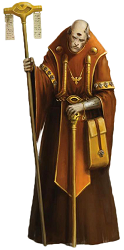
\includegraphics[width=\figwidth]{pics/15/28.png}
	\end{center}
\end{wrapfigure}
The tall and cadaverous man stalked in, probably attracted by all the shouting just a few rooms away from his sanctum, and informed us that we were all blunt-minded idiots. 
No one but Aimy took much offense at this, in our experience the was just the Navigator's way of saying hello, and we all waited to hear why we were bunch of borderline-retards. 
It turned out that what was happening was OBVIOUS, and he could've told us it would've happened if we'd thought to ask him (that statement right there is a classic example of why no one likes Navigators). 
Our ship had just popped out of the warp at an odd location, positively reeked with warp-taint, and had a powerful unrestrained tyranid psychic signature emanating from it; 
the Occurrence Border was a text-book example of a genestealer-infested ship looking to infiltrate a system.

There was a short argument between the Navigator and Tink about whether the Zoanthrope was unrestrained or not. 
Tink ultimately lost, because if the bug was properly restrained we wouldn't have been up to our asses in ghost-tyranids for the last few weeks, but the Navigator did eventually amend his statement to "partially-restrained by bunch of incompetents, heretics, and xenos". 
Anyway, the rest of us acknowledged that this was as good an explanation as any, since excessive paranoia seemed a bit more likely than plain incompetence where the Inquisition was concerned, and asked of the Navigator had any ideas how to deal with such a situation. 
He suggested that we get the hell out of the system before we were all killed, and make sure our next stop was a somewhere where we personally knew people in power who could smooth things out for us. 
This suggestion did not go over well with Doc, Tink, or anyone else really.

\begin{wrapfigure}{O}{\figwidth}
	\begin{center}
		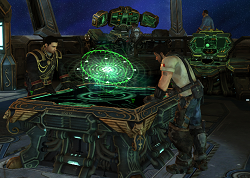
\includegraphics[width=\figwidth]{pics/15/29.png}
	\end{center}
\end{wrapfigure}
In the end, despite all the complaining, Sarge and the Captain decided to follow the Navigator's advice. 
Doc's statement that Gravis would not survive another serious warp journey with the Zoanthrope was noted, as was Tink's list of things in the Cells that desperately needed replacement parts to continue functioning correctly, but those were future problems, and the incoming ships were very current ones. 
Once that critical decision was made, the entire mob relocated to the map-room, where most of us just complained and made unhelpful suggestions while Sarge, the Captain, and our Adepts tried to find a suitable destination.

To our surprise we actually knew a fair number of people who would be able to help us, there was Inquisitor Oak of course, as well as a few of our former Interrogators, an overweight cross-dressing xenophile, the Rupert, and a few tech-priests of various ranks. 
On top of that, the Captain and Adepts were able to supply a few Navy officers and Inquisition contacts, Aimy grudgingly admitted her mother would help if she asked, and Nubby said he knew a guy who was technically a Planetary Governor. 


The problem was that most of these people tended to move around a lot, and the ones who didn't weren't anywhere near our end of the Ultima Segmentum. 
Even without all the complications of making a long warp-journey with Gravis and the Zoanthrope, we just didn't have enough fuel to reach any of them. 
Mind you, if we'd had an Astropath, as opposed to headless corpse in the morgue and a sanctum covered with bits of blood, brain, and bone, we might've gotten lucky and been able to track one of the mobile ones down nearby, but in that case we could've just sent a message asking our boss to sort all this stuff out for us.

\begin{wrapfigure}{O}{\figwidth}
	\begin{center}
		
\includegraphics[width=\figwidth]{pics/15/30.png}
	\end{center}
\end{wrapfigure}
After we examined the map and determined that no one helpful was within our four-day travel range, the Captain raised some less-savory options. 
The discussion turned to what was or wasn't piracy, and whether any of the nearby systems were too small to have naval defenses or astropaths, but developed enough to have a supply of fuel. 


Sarge began to zone out as he imagined just how unpleasant his post-mission interview with the Inquisitor was going to be, and then he overheard Tink pestering the Navigator. 
Tink asked if it was possible to "coast" in the warp like fuel-conscious ships did in normal space, and thereby extend our range enough to reach the nearest guaranteed-friendly system (which was unfortunately the one inhabited by Nubby's "guy"). 
The Navigator made some sneering remarks about a blunt's inability to truly understand the shifting nature of the warp, and admitted that yes, you could trade time for fuel up to a certain point. 


As the rest of us checked whether this would allow us to reach anyone who hadn't been described as "like a Planetary Guv'ner, but wifout da actual planet, and maybe a lil bi' more slavery", Sarge thought back to our original travel plans. 
He asked the Navigator whether we could stretch four days of fuel to reach a destination a week and a half away, specifically the Ordos Xenos Research Facility that had ordered the Zoanthrope. 
He got a flat "No". 
That would've been the end of it right there, and things might have turned out VERY differently, but the Cogitator Adept was listening in, and simultaneously responded with a "Maybe".

That sparked a heated argument, which included a lot of talk about warp currents and something about problems with shortest paths. 
None of us really followed it, except maybe Tink, but the "No" and "Maybe" slowly turned into "Probably, assuming fuel efficiency is static, the currents are where the map says they are, there are no storms, and we can survive three more weeks of Warp travel".

\begin{wrapfigure}{O}{\figwidth}
	\begin{center}
		
\includegraphics[width=\figwidth]{pics/15/31.png}
	\end{center}
\end{wrapfigure}
Well, there was a bit more debate after that, but Sarge had made up his mind. 
He was well and truly done with this shit: 
there would be no more stops, no more hair-raising escapes with misguided Imperial forces hard on our heels, and no more bloody diplomacy. 
He could take three more weeks cooped up with the Zoanthrope and fighting off waves of its ghostly minions, as long as at the end, he'd be able to dump both it and the problem of the crazy Astropaths on whichever Inquisitor had ordered the damned bug.

This decision met a certain amount of resistance, primarily from Doc, Tink, and the Captain, who were tremendously worried about Gravis, the Cells, and the very real chance of running out of fuel short of our destination respectively. 
Unfortunately, despite how undeniably bad Sarge's plan was, no one besides Nubby thought the other options were any better, and anyway, we were Guardsmen and Sarge was in command. 
Once he'd made his decision, all we could really do was complain and try to figure out how to make his plan work.

The Captain went off with his subordinates and the Navigator to plot our route, and informed us that we had five hours before the approaching ships forced us to warp. 
Tink and Jim immediately ran down to the Cells and began frantically working with Fio to overhaul all the stuff they'd originally been planning to replace. 
Sarge, Aimy, and Twitch sat down and began hashing out a defensive plan that would take advantage of the ghost-nids apathy when no one was around to provoke them, and the fact that they didn't ever launch real flanking attacks. 
Nubby dragged Fumbles off to help him relocate several of his stashes to areas that wouldn't be overrun when the shit-storm resumed. 
Doc carefully examined Gravis' condition, evaluated his chances of keeping the Marine alive for three more weeks of warp travel, spent a while locked in the bathroom alternately screaming and crying, and then decided that something drastic needed to be done.

\begin{wrapfigure}{O}{\figwidth}
	\begin{center}
		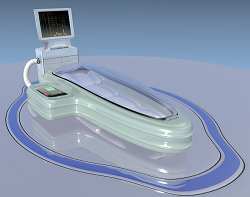
\includegraphics[width=\figwidth]{pics/15/32.png}
	\end{center}
\end{wrapfigure}
Doc made his way down to the Psyker Containment Cells, but thankfully didn't go with his first idea, which had been to just kill the Zoanthrope and hope Oak and his research buddy would be in a good mood when they found out. 
Instead, he poked his nose into the small, currently-unused side rooms that'd originally been used to hold captive psyker children, and checked if any of the undersized stasis-beds had been left over after Tink and Fio had combined a few into one big enough to hold the Zoanthrope. 
He had a moment of panic when all the cells, except for the one packed with debris, were empty, but when he asked Fio what had happened, the little xenos explained that they'd pulled them all out during the project and the leftovers were just in a closet somewhere. 
Doc knew the inevitable fate of expensive pieces of equipment that got left in unmonitored closets, so he skipped the scavenger hunt and just commed Nubby to ask which one of his stashes the stasis beds had wound up in.

Nubby wasn't keen to part with his loot, but eventually came around to Doc's way of thinking when the Medic started explaining all the horrible things that would happen to him if Gravis died. 
One of the five leftover stasis beds was hauled up to the medbay, where Doc and Valerie spent several minutes trying to figure out how to fit the upper half of a three-meter tall killing machine into a stasis bed sized for children ages 3-12.

It was obvious from the start that Gravis' armor and life support machinery wouldn't fit, but it was quickly established that even without those, he was still far too large. 
In the end Doc was forced to admit that the only way it would work was if they removed Gravis' arms, shoulders, and a good portion of one of his sides; 
Sister Valerie did NOT approve of this course of action.

\begin{wrapfigure}{O}{\figwidth}
	\begin{center}
		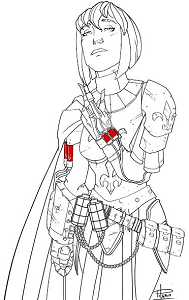
\includegraphics[width=\figwidth]{pics/15/33.png}
	\end{center}
\end{wrapfigure}
There was a short argument between Doc and his girlfriend over whether being slowly hacked apart with a diamond-edged bonesaw while struggling to fight off an alien biotoxin was guaranteed to be fatal or not. 
Nubby, who'd tagged along in hopes of getting his loot back, decided to be helpful at this point, and suggested that Gravis didn't need to be cut up before going into the bed, as the stasis field could take care of it for them. 
He was in the middle of rather gleefully recounting what had happened to a cargo-servitor that'd been caught half in a field during Tink and Fio's experiments on combining stasis units, when Doc realised the obvious solution to the problem.

A few minutes later, Doc was down in the Cells screaming at Tink to stop messing around with the psi-suppressors and get to work combining the five leftover stasis beds into one large enough to hold Gravis. 
Tink was pretty sure that his current task was a little more important though, so there was a bit of an argument, and things quickly devolved to the point where Doc was holding techie up by the collar and shaking him. 
Jim stepped in that point, applied a few thousand volts of enforced calmness to Doc's lower back. 
He explained to the twitching medic that his request had been noted, but building the stasis unit would take a few days, and would therefore have to be worked into the schedule between critical maintenance on the Cells.

Doc was in no position to argue with Jim, or walk for that matter, so he accepted the cogboy's promise that it would be a top priority, and was dragged back to the medbay by Nubby and Fumbles. 
He felt slightly better when Sister Valerie called him a genius and promised to kiss him later, when she wasn't covered with bodily fluids.

Two hours later we sent out a final message to everyone in the system, which was pretty much a detailed list of why they were all idiots and/or assholes, and disappeared into the warp before the approaching ships could follow us.

\begin{wrapfigure}{O}{\figwidth}
	\begin{center}
		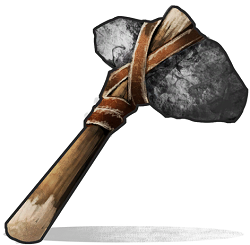
\includegraphics[width=\figwidth]{pics/15/34.png}
	\end{center}
\end{wrapfigure}
All you could really say for the first few days of that warp journey, was that they went better than the last few of our previous one. 
For a starter, our worst-case scenario (for conservative values of "worst") hadn't come true: 
the ghost-nids hadn't just popped back into existence in the same places they'd been when we'd dewarped. 
Our brief stint in normal space had reset their counter or whatever, and the bugs were only appearing in the tainted areas, though at a rate significantly higher than they had before. 
Spawn rate aside though, our defensive situation was MUCH better than it had been, and the Cells were in pretty good condition too. 


Thanks to the heroic repair efforts of Tink, Jim, and Fio, the psi-suppressors took the strain of entering the warp without failing, and the devices seemed to be functioning better than they had before. 
There were some concerns about their power output though, since as mentioned, the ghost-nid spawn rate was higher than it had been, and there were also more minor phenomena occurring throughout the ship as well as an increase in the number of IGPs (Inexplicable Gravis Problems). 
This bothered Tink immensely, since his readings said everything in the Cells was working fine (at least for now), and there wasn't any psychic leakage around the Cells either. 
Admittedly Fio and Jim's psi-detectors consisted of the Wraithbone block on a stick and a creepy ornate servo-skull that had to be periodically fed live rats, but they seemed pretty confident in their readings.

Anyway, Tink and the other techies didn't get to ponder the ghost-nids for long. 
Even though the normal-space repairs had bought them some breathing room, the lack of replacement parts meant every fix they made was a horrible time-consuming kludge, and Doc made sure that every minute of their free time was dedicated to putting together Gravis' stasis field.

\begin{wrapfigure}{O}{\figwidth}
	\begin{center}
		
\includegraphics[width=\figwidth]{pics/15/35.png}
	\end{center}
\end{wrapfigure}
Things were more-or-less calm for the first three days of our efficiently-slow warp journey. 
We kept track of the ghost-nids, but didn't waste any effort engaging them, Tink and Fio managed to make some serious progress, and Doc managed to stay very positive about the situation while struggling with Gravis' mounting medical problems. 
The first suppression failure happened on the fourth day.

The increase in phenomena and ghost-nid spawning was pretty much a repeat of the last time, but the other aspects of the failure went differently. 
For one thing, we didn't lose any armsmen on account of how ghost-nids still hadn't expanded to reach our defensive lines when the failure began, they sure as hell had reached them by the end though. 
This time Fumbles did better too, he managed to retain consciousness through the whole thing, though he was a little loopy afterwards, babbling about something being "all around" and "trying to find itself". 
Gravis, however, came off a lot worse: 
Doc and Valerie weren't able to figure out exactly what had happened, but the Space Marine's secondary heart wound up resembling a raisin, and had to be removed. 
Once again, the techies managed to fix things, but that marked the end of the easy part of the trip.

As the fight against the ghost-nids resumed, we realized that their spawn rate wasn't the only thing that'd gotten worse over time. 
The bugs were definitely stronger and more aggressive than they had been during the last trip, and they began to exhibit some new and worrying behavior. 
Three times in the following two days sizable forces of ghost-nids coalesced in areas where they hadn't reached our lines yet, and then slowly wandered into the ship until they ran into our forces. 
We managed to beef up the defenses in time on all three occasions, but they were all difficult fights, and this change in attack patterns forced Sarge, Aimy, and the Captain to seriously re-evaluate their plans.

\begin{wrapfigure}{O}{\figwidth}
	\begin{center}
		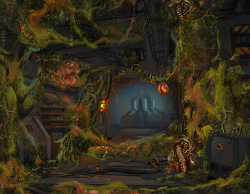
\includegraphics[width=\figwidth]{pics/15/36.png}
	\end{center}
\end{wrapfigure}
By the sixth day it was becoming apparent that holding out for two more weeks would be close to impossible. 
The unexpected increase in the ghost-nids' strength and their new penchant for the occasional focussed attack forced our lines back days ahead of schedule, and the initial ship-wide increase in phenomena we'd seen was getting worse. 
It was actually beginning to feel like the Gellar field was failing, except Ol' Bill was certain it wasn't, and the usual whispers and blood-seepage had been replaced with far-off chittering sounds and tyranid-ichor. 
It was obvious the Zoanthrope was responsible, but it was still a mystery how, and we couldn't think of anything to do about it besides killing the bug or dewarping.

Mind you, dewarping wasn't the same sort of emergency option it'd been before. 
This was because the warp-drive took a whole lot of energy to function, so we didn't actually have enough fuel to get back into the warp of we exited, much less go anywhere or dewarp again afterwards. 
So if we wanted to bail out of the warp, we were going to need to do it near a system that could provide fuel, and handle all the risks that came with that. 
Still, the situation with the ghost-nids was getting bad enough that Sarge was really considering calling for a detour, though the only chance coming up to do so was at least another three days of warp-current coasting away.

So the situation was bad, but there was at least one bright spot: 
thanks to the time freed up by a lucky streak of only minor malfunctions in the Cells, Tink and Fio had nearly completed Gravis' stasis field. 
In fact they were down to just the last little part, dealing with the power-distribution, and it was proving rather tricky. 
Since they didn't want to waste time doing it all from scratch, the two of them went down to the Cells to take a hard look at how they'd done it last time. 
That turned out to be a VERY good decision.

\begin{wrapfigure}{O}{\figwidth}
	\begin{center}
		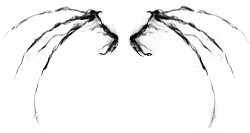
\includegraphics[width=\figwidth]{pics/15/37.png}
	\end{center}
\end{wrapfigure}
Now, despite the Zoanthrope being the focus of all this trouble, the three techies didn't actually pay that much attention to it most of the time. 
For one thing, after Tink'd fixed the flickering problem, its stasis field had been working surprisingly well; 
it was always the devices scattered around the room that needed maintenance. 
Secondly, the Zoanthrope had gotten incredibly creepy after Sarge's slagged hull-metal shield had gotten wrapped around its head. 
It never moved obviously, being in stasis and all, but you always felt it was watching you under the metal, and the longer you looked at it the worse it got. 


In retrospect that was probably what some fancy-pants Inquisitory Super Agent Guy would've called a "clue", but we were a little too busy for that shit. 
We just accepted that the metal-faced xenos psyker that looked like a cross between a fetus, a snake, and a cockroach was creepy, and felt no need to examine said creepiness for a supernatural element.

Anyway, all this meant that, when Tink crawled under the stasis unit to poke around and asked Fio to watch the field for any flickers, it was actually the first time anyone had really looked hard at the Zoanthrope since we'd re-entered the warp. 
After a minute or so, Fio asked Tink if he'd touched anything, and when the techie replied in the negative, the little Tau scientist explained that there was some sort of interference pattern inside the field. 
Tink looked at the focusing array above his head, which looked perfectly intact to him, and asked what the pattern had looked like, and whether it might be yet another psychic phenomena. 
Fio walked a circuit around the stasis unit, turned his head from side to side, and reported:

\greentext{>There's actually two focal points, both positioned right behind the Zoanthrope. They're sort of black and smoky, and shaped like little… wings?}


\begin{wrapfigure}{O}{\figwidth}
	\begin{center}
		
\includegraphics[width=\figwidth]{pics/15/38.png}
	\end{center}
\end{wrapfigure}
So no shit, there we were, in the middle of the warp, too low on fuel to even consider stopping, when we realized our captive ghost-summoning insectoid xenos psyker, was actually a ghost-summoning insectoid xenos DAEMONHOST. 


I mean… what the hell? 
Seriously. 
Just how in the name of the Emperor are you supposed to respond to something like that? 
There's bad situations, and then there's comically bad situations…

Anyway, it actually took us a little while to figure out that the Zoanthrope was possessed. 
None of the techies knew much about daemons, and of the three of them, only Jim had been on the Occurrence Border during its maiden voyage as an Inquisitorial vessel and he hadn't actually encountered the daemon that had eventually possessed the Cogtain. 
So the three of them gawked at the Zoanthropes miniature smoky wings for a while, debated whether it was something that could be ignored, and eventually commed the rest of us to ask if we had any ideas what was going on.

According to the armsmen fighting alongside Sarge, his swears were so vitriolic that they actually turned into little insectoid creatures as they left his mouth, and had to be swatted out of the air as they tried to bite people. 
Given how warpy his section of the line had gotten by that point, none of us questioned this. 


Doc burst into hysterical laughter when he heard. 
This caused a little bit concern among the medical staff, especially the two nurses who'd seen him melting people with Tyranid biotoxin. 
Sister Valerie carefully relieved him of his scalpel, dosed him with something relaxing but not incapacitating, and took over Gravis watch while he giggled his way down to the Cells to see the wings for himself.

After a brief period of mindless panic, Nubby denied all responsibility for what had happened, and then had to explain to those of us who hadn't been there what exactly wasn't his fault.

Twitch just screamed "I TOLD YOU IT WAS DAEMONIDS" into his combead until Tink muted him.

\begin{wrapfigure}{O}{\figwidth}
	\begin{center}
		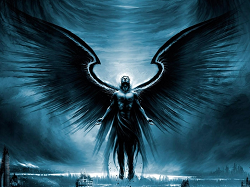
\includegraphics[width=\figwidth]{pics/15/39.png}
	\end{center}
\end{wrapfigure}
Over the course of the next few hours everything that had been happening started making sense.

There was some initial confusion about how it was all possible, since the Xenology Adept kept telling us absolutely could not possess Tyranids. 
He gave this big lecture on how the Hive Mind worked then trotted out that old line about Nids not having minds or souls (though anyone who's seen a Daemon Engine stomping around a battlefield can tell you neither of those are strictly required). 
Anyway, the man was obviously full of shit: 
I mean, we could all see the wings, just sitting there being all smoky and sinister, if a bit on the tiny side. 
Can't really argue with that. 


So, whether it was a matter of a dozen unimaginable coincidences coming together to make the impossible possible, or if the Emperor had just decided to screw with us, we had the first known case of a possessed Tyranid sitting in the Cells. 
We hoped Oak's research buddy would be happy with it, because we weren't going to go back and get another one.

Where the daemon had come from was a little more clear. 
Back during our first trip on the Occurrence Border, we'd come down to the Psyker Containment Cells and found them occupied by five child psykers in stasis, and a half-pint daemonhost who wasn't. 
After we looted a crucial part of the machinery restraining the daemonhost (as well as the five non-possessed children), the thing had chased us across the ship. 
It had looked like a kid with massive wings made of smoke, curly horns, and glowing eyes, at least until we shot its host body to pieces and it ran off to get a new one. 


The daemon came back a little later as a knarloc with the same wings and such, and had then gotten tangled up in a fight with a giant daemonic-servitor-titan thing that the tech-priest acting as the ship's Captain had been constructing for whatever insane reason. 
That had ended with the knarloc being incorporated into the servi-titan and daemon taking over the Cogtain.

\begin{wrapfigure}{O}{\figwidth}
	\begin{center}
		
\includegraphics[width=\figwidth]{pics/15/40.png}
	\end{center}
\end{wrapfigure}
It took some doing, but we eventually destroyed the servi-knarlo-titan, pitched the Cogtain into the bridge-lift's shaft, and cranked the gravity up as high as it would go. 
That'd done for the Cogtain, and between reducing its host to a greasy crater and our subsequent exit from the warp, we'd assumed that was last we'd seen of the smoke-winged daemon as well. 
The fact that the Cogtain's crater could never be repaired, even  by replacing entire sections of floor and wall, and the way it screamed at people in binary probably should've tipped us off.

So we'd dismissed the glowing, screaming crater as just another Occurrence Border thing (trust me, it doesn't sound stupid after you've been on the ship for a while), and got on with our lives. 
It didn't come to our attention again until we began refurbishing the Cells in preparation for the Zoanthrope, and had discovered that there was some sort of daemonic portal linking the cell that'd held the daemon's first host to the crater. 
Once again we dismissed it as just another phenomena, and pretty much forgot about it. 
In retrospect, even without the daemonic involvement, it should've occurred to us that having some sort of warp-portal INSIDE of all the psi-shielding and warp-presence shrouding was a very bad thing.

Not being daemonologists, we had no idea whether the daemon had been lurking in the cell or crater all this time, or if it had actually returned from the warp via the places it had tainted. 
Either way, the presence of a restrained and frequently unconscious psychic being, with no Emperor or Hive Mind to protect it, must have looked incredibly tasty to it. 
The daemon had probably been slowly corrupting the Zoanthrope ever since we caught it (How does that work with a giant bug anyway? 
Does the daemon tempt it promises of sugar or something?), but we felt fairly certain that the that Sarge knocking the Zoanthrope out consciousness and into the tainted cell had been the final straw.

\begin{wrapfigure}{O}{\figwidth}
	\begin{center}
		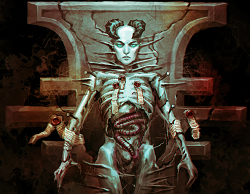
\includegraphics[width=\figwidth]{pics/15/41.png}
	\end{center}
\end{wrapfigure}
After we'd figured out that we were dealing with (as Twitch put it) a Daemonthrope, and one that was sort of connected to this warp-portal which bypassed all of the psi-shielding around the cells to boot, all the stuff with the ghost-nids made sense. 
Well sort of, we still didn't know what exactly they were, but at least it was clear how they were being called into existence despite the Zoanthrope being contained in the cell. 
None of us were experts on imprisoning daemonhosts, but we were pretty sure it took a bit more than a few psi-suppressors and a stasis field to do the job properly.

Of course knowing that you're doing something wrong isn't the same as knowing how to do it right. 
The Inquisition had always operated under the assumption that daemon-lore was a very need-to-know subject, and in the Inquisition's opinion a bunch of dumb grunts most certainly did NOT need to know. 
Mind you, up until this shit-show we'd agreed with that assessment. 
None of us had ever imagined that we'd wind up trying to prevent a daemonically possessed psychic bug from summoning tides of ethereal tyranids, or at least not without just killing the damned thing and calling it a day. 
Anyway, the point is that our team's combined knowledge of daemon-binding (or whatever you call it) consisted of a suspicion that it probably involved a bunch of runic circles, holy icons, and sinister looking chains that weren't actually connected to anything load-bearing. 
The key words there were "suspicion" and "probably" by the way.

So lacking even the slightest idea how to handle the Daemon directly, we decided to hope like hell that dealing with the source of the problem would somehow fix everything. 
All of our highly developed problem solving skills were focused on the daemonically tainted cell, and a complex plan of action was formed. 


Which is to say that we set up a blast shield and tossed half a dozen detpacks into it.

\begin{wrapfigure}{O}{\figwidth}
	\begin{center}
		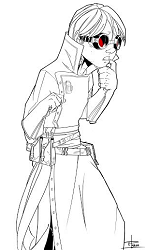
\includegraphics[width=\figwidth]{pics/15/42.png}
	\end{center}
\end{wrapfigure}
Of course the "just blow up the daemonic portal" plan didn't work, but y'know it MIGHT have, and it would've been really silly not to check. 


So, after establishing that all we'd managed to do was severely damage the shrine surrounding the Cogtain's crater and scare the shit out of a bunch of tech-acolytes working on the bridge-lift, we moved on to our next low-effort solution. 
We took one of our three spare pieces of psi-shielding, crammed it into the doorway to the tainted cell, and then slapped a few dozen prayer seals on it. 
When that didn't work we added the two other pieces of shielding, and when THAT didn't work, we finally allowed Fumbles to take a look. 
That was a nervous ten minutes, let me tell you.

Despite our very well-founded concerns, letting the accident-prone psyker poke at the daemonic warp-portal worked out fine. 
Mostly because the psi-suppressors kept him from doing anything when he eventually spazzed out. 
Afterwards, once Fumbles had been woken up, and Twitch had stopped abjuring him and throwing holy water around, the psyker blearily reported that nothing we were doing actually had any effect on the flow of daemonic energy between the tainted cell and the Daemonthrope. 
However, he was reasonably sure that increasing the distance between to two would at least reduce the flow a bit. 
Since moving the warp-portal wasn't an option, the only way to accomplish this was by moving the Daemonthrope, plus the various pieces of technology which kept it from killing us all.

The task of figuring out how to more or less relocate the entirety of the Cells fell to Tink, who immediately declared it to be impossible. 
This didn't stop him from calling a council of the nerds, including Ol' Bill and Hannah, to figure out exactly how impossible it was though.

\begin{wrapfigure}{O}{\figwidth}
	\begin{center}
		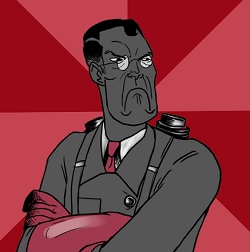
\includegraphics[width=\figwidth]{pics/15/43.png}
	\end{center}
\end{wrapfigure}
Tink and his little think-tank quickly established that the only system in the Cells that could be easily moved was the psi-suppression. 
This was primarily because they'd stopped bothering to bolt the suppressors back down between maintenance cycles, so they were all just taped to the floors and walls. 
On the other hand, the psi-shielding and warp-presence Shroud, which Fumbles said were hiding the Daemonthrope's location from its ghost-nids, were pretty much built into the structure of the Cells. 
Just removing them would require days of cutting, during which the ghost-nids would probably swarm the Cells. 
Finally, the stasis-unit restraining the Daemonthrope was NOT designed to be moved. 
Jostling the focusing array could cause problems ranging from flickers to spontaneous bisection of anything inside the stasis field, and power efficiency hadn't even been considered in its design so running it off a battery was going to be tricky.

The first problem to be solved was the stasis field. 
Tink and Fio realized that they didn’t have to fix everything wrong with the Daemonthrope’s stasis unit, since they had a much-better one sitting nearly-finished, just a few rooms away. 
Their decision to repurpose Gravis’ stasis unit almost got the two of them stabbed by an enraged medic, but luckily they were able to propose a solution for keeping Gravis alive as well. 


Tink explained, from behind an overturned table, that there was no reason that the nearly-dead Space Marine couldn’t just be thrown into the Daemonthrope’s stasis unit after the bug had been relocated. 
Doc had not been happy with leaving his patient, even in stasis, next a daemonically-tainted hole in reality, but eventually agreed and allowed Tink to flee the medbay.

\begin{wrapfigure}{O}{\figwidth}
	\begin{center}
		
\includegraphics[width=\figwidth]{pics/15/44.png}
	\end{center}
\end{wrapfigure}
The psi-shielding and the Shroud were much trickier problems, and a fair bit of time was spent lamenting that the whole mess at the Station had ruined our original plans to requisition enough materials to completely rebuild the Cells. 
After a few hours of trying to figure out how to pull everything out and set it back up before a tide of ghost-nids killed everyone, the ludicrous proposal of cutting a massive hole through the ship, and moving the Cells (minus the warpy bit)  as one big-ol' thingy was put forward. 
Luckily Ol’ Bill saved us all from that retarded plan when he decided to take a second look at the list of parts that'd need to moved.

Consummate scrounger that he was, Ol' Bill could typically suggest five different alternatives for any missing critical part, and he was better than a savant when it came to keeping track of what had be used where and whether it would be missed. 
His abilities had let him down a little bit when it came to the highly-specialized systems in the Cells, but they came to our rescue in a big way when he asked whether a psi-shield panel was anything like a psi-focussing panel. 
After some debate, Tink pointed out that it was all moot, since there weren't any psi-focussing panels in the inventory; 
Ol' Bill asked whether anyone thought our headless astropath still needed the ones lining his sanctum.

One quick check of the dried-brains-splattered sanctum later, it was established the panels which focussed incoming astropathic messages on the chair in the middle of the sanctum could indeed be repurposed as shields. 
Fio, who'd become the resident expert on the underlying theory of most of the systems in the Cells, claimed it was just a matter of tweaking the machinery that aligned the crystal matrices in each panel, and began estimating how long it would take to move them all the bay that'd been picked for the new Cells. 


Tink asked why the hell we should bother moving them.

\begin{wrapfigure}{O}{\figwidth}
	\begin{center}
		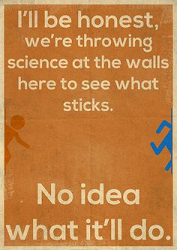
\includegraphics[width=\figwidth]{pics/15/45.png}
	\end{center}
\end{wrapfigure}
The decision to just repurpose the Occurrence Border's bridge-adjacent Astropathic Sanctum as a Daemonthrope holding area was reached quickly by Tink and his fellow nerds. 
It took a little more time and a LOT more shouting for Sarge, the Captain, and the Navigator (whose sanctum was next door) to come around, and that time was used to tackle the final problem: 
the warp-presence Shroud.

The Shroud was a device which hid the warp-presence of anyone inside from those outside. 
Such devices were typically used to hide vulnerable psykers from hungry daemons during warp-travel, but they were also great for hiding from other psykers. 
Since the Occurrence Border had been smuggling child-psykers, a practice which the Inquisition SORT OF frowned upon, the Cells had a very good Shroud, though it hadn't done jack to hide the Zoanthrope from the daemon that'd been lurking inside its radius. 
Anyway, this well-made Shroud consisted of a fair-sized pile of arcane machinery which was unfortunately hooked to some sort of projector matrix embedded in the psi-shields.

Once again it seemed like days of disassembling while fighting off a ghost-nid onslaught would be needed, but Fio had a better idea. 
The little Tau scientist claimed that the block of wraithbone he'd been playing with for the last few weeks had some interesting anti-warp properties, and he was 72.361% sure that it could be used to build something that would work like a Shroud. 
It was a mark of everyone's exhaustion that the annoying little xenos' idea was accepted without argument.

So roughly twenty-six sleepless hours after our discovery of the Zoanthrope's wings, we'd designed a new Cell to contain it. 
Thirty hours of hard work and heroic ghost-tyranid killing after that, the new cell was complete, and all that was left to do was transport the barely-restrained xenos daemonhost through a ship filled with the ravenous insectoid warp-ghosts it'd called into existence.

\begin{wrapfigure}{O}{\figwidth}
	\begin{center}
		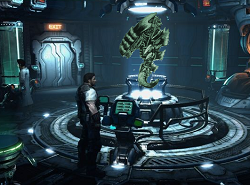
\includegraphics[width=\figwidth]{pics/15/46.png}
	\end{center}
\end{wrapfigure}
When Tink said everything was ready, all of us plus Fio, and Gravis' mobile medical monstrosity gathered in the cells. 
During the prior few days we'd managed to hold off ghost-nids and keep the Space Marine alive despite a steady increase in the Daemonthrope's power over the ship and the irreparable failure of one of the psi-suppressors. 
During the little free time we'd had, a route had been plotted from the Cells, up through the lower decks to the bridge-lift, and finally to the Sanctum. 
The corridors were cleared of impediments, all the armsmen that could be spared from the main lines were stationed at checkpoints along the route, and the new stasis unit had been mounted on a motorized cargo pallet. 
When the last of the preparations were finished, Sarge alerted the Captain, who sent out a ship-wide warning, and we got ready for the most hectic prisoner transfer of our lives.

The first step of transfer was moving the Daemonthrope from its old stasis unit to the new mobile one. 
There's probably a whole chapter on this sort of thing in whatever the Inquisitorial equivalent of the Uplifting Primer is. 
You're probably supposed to use all sorts of seals, powerful psykers, and some of that special Tyranid tranquilizer the Scythes had. 
We made do with a few ropes, a ramp made out of a wall-panel that no one would miss, and a cargo net.

Tink lined up his long-distance manipulation tool (see: 
poking stick) on the Stasis Unit's Off-Button, then jabbed it and dove for cover. 
As the stasis field vanished, a pair of deep-red spots appeared on the Daemonthrope's metal-covered face, and its stubby little smoke-wings suddenly expanded to a full meter in length. 
A horrible soundless screech echoed through the Cells, thousands of insects began pouring out of every crack and crevice, and a corona of black-edged green lighting formed around Daemonthrope. 
Then the cargo net yanked it off its grav plates, and dragged it face-first down the corrugated metal ramp.

\begin{wrapfigure}{O}{\figwidth}
	\begin{center}
		
\includegraphics[width=\figwidth]{pics/15/47.png}
	\end{center}
\end{wrapfigure}
The Daemonthope flailed around a little, but didn't have enough strength to offset the manly (and womanly) muscle of four guardsmen. 
We dragged it, screeching and kicking up sparks, into the waiting stasis unit, and Fio turned on the field. 
The insects around the room vanished in little puffs of black and green smoke, but a faint echo of the psychic screeching lingered, and the spots where the Daemonthrope's expanded wings met the edge of the stasis field smoked in an ominous way. 
Sarge decided that this shit was too eldritch for his liking yelled at Tink, Fio, and Doc to move their asses.

Doc was in a bit of a panic on account of how insects had been crawling out of Gravis' torso-wound during the Daemonthrope transfer, and the fact that every life-support system hooked up the Marine was screaming for attention. 
He dithered around trying to figure out what to treat first, until Sarge resolved things by hefting Gravis off his life-support bed. 
Doc tried and failed to keep everything connected as the torso-fied Space Marine was hauled across the room, then just gave up and helped Sarge. 
Gravis started to spasm and spurt all sorts of disgusting fluids as he was pushed into the bubble of null-g in the middle of the stasis unit, prompting Doc to panic and hit the On-Button a little early. 
He apologised profusely as he bandaged Sarge's slightly-shorter finger, and sprayed disinfectant over everything Gravis had dribbled on.

While Gravis was moved, Tink and Fio ran around directing us and their drones in the process of moving the psi-suppressors. 
Extensions were spliced into the power cords of each of the hacked-together Tau-Imperial hybrid devices, and a jumbled circle of arcane machinery was formed around the Daemonthrope's stasis-pallet. 
Then, piece by piece, each of the psi-suppressors was fastened to the pallet, until it bristled with various engines, antennas, crystals, and less-identifiable pieces of tech.

\begin{wrapfigure}{O}{\figwidth}
	\begin{center}
		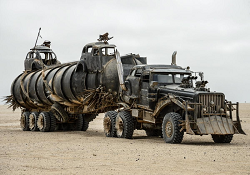
\includegraphics[width=\figwidth]{pics/15/48.png}
	\end{center}
\end{wrapfigure}
When all the suppressors were fastened down and connected to the large battery array mounted on the front of the pallet, and Gravis was safe-ish in the Daemonthrope's old Stasis Unit (we were pretty sure that his expression of pain and horror wasn't anything to worry about), we readied our weapons and got ready for the hard part. 
Sarge sent a final warning to the Captain, and counted down. 
As Sarge reached zero, Spot 2.0 opened the outer door to the Cells, and all across the ship the tyranid warp-ghosts paused in their pursuit of re-positioning armsmen, turned to focus on us, and solidified. 


We came out of the Cells at a dead sprint, or at least those of us on foot did. 
Fio was perched in a semi-clear spot on the Pallet behind the Daemonthrope, gibbering at his drones in Tau-speak and doing his best to keep everything from spontaneously exploding. 
Tink had a similar spot on battery-pack, and was splitting his attention between steering the Pallet and scouting ahead with Spot. 
Twitch and Sarge were on point, pulling ahead to cover each corner and doorway. 
Aimy and Doc were keeping an eye on our flanks from the middle of the group. 
Finally Nubby was squeezed into a crevice at the back of the Pallet, where he was simultaneously able to cover our rear and avoid doing any running.

To our immense relief, we made it to the end of the corridor without the Daemonthrope doing anything warpy or a swarm of ghost-nids just appearing around us. 
Tink and Fio had said that leaving the Cells wouldn't suddenly grant the Daemonthrope more power, but the rest of us hadn't been so sure. 
Anyway, after that first straightaway we began winding through the area around the Cells in a manner that could be described as "drunken". 
Despite all appearances though, it really was the fastest route available.

\begin{wrapfigure}{O}{\figwidth}
	\begin{center}
		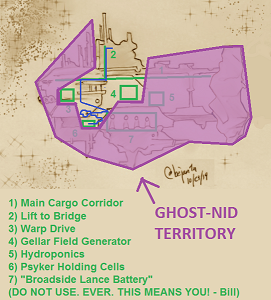
\includegraphics[width=\figwidth]{pics/15/49.png}
	\end{center}
\end{wrapfigure}
Due to the chaotic layout of the Occurrence Border, the size of the Pallet, and the amount of the ship occupied by the ghost-nids, the path we'd mapped to the Sanctum was anything but direct. 
The first leg involved a winding path around the Cells area, which took us dangerously close to ghost-nid territory before depositing us at one of the few major "tilt-corridors" still under our control. 


We ran as fast as we could through connecting corridors, across recently cleared storage bays, and up the occasional micro-lift, ignoring the various minor phenomena, maddening whispers, and occasional uncleared technical hazards. 
Our progress was surprisingly good, possibly because we were lent extra motivation by what sounded like every ghost-nid on the ship baying for our blood, but it wasn't enough to keep us ahead of the entirety of the swarm: 
the first pack of ghost-nids clawed its way out of an oversized air vent behind us as we exited a short in-bay lift.

Luckily that first pack hadn't included any ghostly termaguants or higher forms: 
it was just a bunch of hormagaunts and rippers, though they were significantly more solid than any we'd encountered during the previous weeks. 
Solidity aside, we knew how to deal with a bunch of melee hostiles coming up a cover-less corridor. 
Nubby began picking off the lead bugs with pulse fire, while Twitch dug through his detonators, and the rest of us kept moving. 
As the bulk of the pack passed a pair of yellow X-marks on the corridor wall behind us, Twitch found the right detonator, and set off two of the frag-mines he'd lined the corridor with. 
Doc and Aimy paused for a second to help Nubby mop up the stragglers, and then everyone returned to their positions and our flight continued without the Pallet ever losing any speed. 
As the last of us left the corridor, Twitch armed the rest of the mines, and a minute later we heard them start going off.

\begin{wrapfigure}{O}{\figwidth}
	\begin{center}
		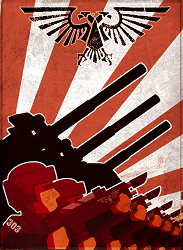
\includegraphics[width=\figwidth]{pics/15/50.png}
	\end{center}
\end{wrapfigure}
Variations of that little scuffle were repeated a dozen times as we escorted the Daemonthrope towards the checkpoint at the start of the tilt-corridor. 
The ghost-nids were harder to kill than any we'd encountered during the previous weeks, they took just as much killing as real tyranids despite the way they poofed into smoke when they finally died. 
On the bright side, the bugs' new solidity seemed to have robbed them of their ability to move through walls, though they made up for it with a freakish ability to home in on us. 
Wave after wave of the bugs came up behind our little convoy, as well as through the vents on the walls and ceilings, and eventually from ahead of us as our course turned back towards the ghost-nid territory. 


The continuous attacks slowed us down a little, but didn't pose a serious threat: 
they were just Gaunts and Rippers after all, and we were bloody Imperial Guardsmen. 
Mowing down endless waves of under-armed xenos with superior firepower is what the Emperor made us for. 
Between Twitch's mines, the early warnings and target marking from Spot the Wonder Drone, and giant pile of pulse-ammo we'd brought along, we dropped most of the nids the second we saw them. 


Of course that's not to say that EVERYTHING went our way: 
either the Daemonthrope was exhibiting some serious power despite its stasis-ed state, or the Occurrence Border's warpy little machine-spirit had a really twisted sense of humor. 
On four occasions during our twisty run towards the checkpoint at the bottom of the tilt-corridor we ran into phenomena that seemed specifically designed to either slow us down or assist the ghost-nids in killing us.

\begin{wrapfigure}{O}{\figwidth}
	\begin{center}
		\includegraphics[width=\figwidth]{pics/15/51.png}
	\end{center}
\end{wrapfigure}
Two of the delays were frustrating, but non lethal in and of themselves. 
Twice, immediately after Spot had flown through a doorway, it slammed shut, and re-opened on an all-too-familiar giant room filled with fire when we reached it ourselves. 
The first time it happened Twitch led us on a winding detour which had involved several ghost-nid attacks in tight corners, the second time Tink just plasma-ed us a new door next to the fiery one.

The Daemonthrope, or maybe just our terrible luck, struck again at the midway point of that first leg of our journey, when we all simultaneously ran out of breath and were deafened by a shill and chittering keening sound. 
It wouldn't have been that much of a problem, except for the fact that it coincided with attacks from our front and rear by waves of gaunts. 
The sudden slowdown and inability to communicate might've been lethal for our exposed pointmen if the rest of us hadn't been on our toes. 
Doc and Aimy, operating completely independently, both tossed frags at the pursuing swarm, and grabbed a hold of the motorized Daemonthrope pallet right as Tink floored it and Nubby took care of the stragglers. 
They arrived just a little too late to prevent the frontal attack from reaching Sarge and Twitch, but Sarge was a big boy who could handle a few scrapes and scratches, and Twitch had just hidden behind the beefy noncom until relief arrived.

The final serious phenomena occurred only two rooms from the checkpoint, and very nearly got us all killed.

\begin{wrapfigure}{O}{\figwidth}
	\begin{center}
		\includegraphics[width=\figwidth]{pics/15/52.png}
	\end{center}
\end{wrapfigure}
We were crossing a storage bay that apparently held tanks of drinking water, headlight fluid, pressurized liquid chlorine, and toothpaste, when a pack of ghost-nids clawed a hole through a door on Aimy's flank. 
As she started picking the bugs off, a sort of howling spectral gale manifested in the corridor behind the bugs, and three of them were propelled through the hole like angry insectoid cannonballs. 
One gaunt was shot out of the air, another pancaked against the toothpaste tank, and the third landed on Aimy.

Aimy's panicked snapshot missed the gaunt, passed a centimeter in front of Fio's face, and exploded one of the crystal-tipped suppression pylons mounted on the Daeomonthrope's pallet. 
The lights abruptly went out, frost began to form along the walls, and the bay's vox system began screaming at us in a mix of Jantine Battle-Cant and Hrud. 
 All of us except Aimy, who was trying to keep the gaunt from eating her face, and Nubby, who helpfully shot it off her, activated our tac-lights and scanned the room for any sort of new warpy threat while Fio tried to repair the suppressor and Tink kept the pallet moving. 
Our rubbernecking was brought to an abrupt halt by three sudden realizations. 
Firstly, that the ghost-nid on top of Aimy was reforming instead of dissipating into smoke. 
Secondly, the screaming vox was just a leakage alarm as opposed to some sort of warp phenomena. 
And finally, that Aimy's shot had terminated in the pressurized chlorine tank.

Aimy practically teleported out from under the reforming gaunt, which Nubby shot a few more times for good measure, and we bailed out of that bay so fast that we literally stampeded the nids coming at us from ahead. 
As we exited Doc attempted to close the bay behind us, only to find a little yellow note apologizing for scrounging the door's control panel. 
He settled for tossing a nade at the now-reformed gaunt and the other nids that were moving through the gas with impunity.

\begin{wrapfigure}{O}{\figwidth}
	\begin{center}
		\includegraphics[width=\figwidth]{pics/15/53.png}
	\end{center}
\end{wrapfigure}
We hit the tilt-corridor checkpoint at a dead sprint with the ghost-nids and gas hard on our heels. 
It took the armsmen defending the barricade-packed fourway junction a few seconds to register our presence, which was understandable given the way the bugs they were holding off had started reforming as we approached. 
When the sergeant-at-arms leading the group finally realized we were there, he nearly put a round in the Daemonthrope out of sheer reflex, but Sarge caught him in time, and started belting out orders.

Our initial plan had been to take a breather, restock on ammo, and swap out the Pallet's batteries for the ones we'd stashed here, but the reforming nids and the inexorably approaching gas-cloud meant there wasn't time. 
Each of us grabbed what we could in the the ten seconds it took Sarge to order the armsmen to get ready to bail, preferably to somewhere airtight, and Tink coupled the pallet to the cart-thing waiting at the edge of the tilt-corridor. 
Fio, still busy trying to fix the psi-suppressor Aimy had shot, screamed at the tech-acolyte holding the replacement batteries to just hop on the cart, and followed the terrified cogboy aboard. 


An entire thirty seconds after our arrival, the armsmen manning the barricades beat feet. 
By the forty second mark, a mix of chlorine gas and warp-spawned tyranids had filled the checkpoint. 
Ten seconds after that, the detpack Twitch had left on the pile of leftover ammo turned the whole place into a gas and gore filled crater. 
We would've stopped to high-five each other, but we were a little too busy holding on for dear life as we raced down (or up, depending on how you looked at it) the tilt-corridor.

\begin{wrapfigure}{O}{\figwidth}
	\begin{center}
		\includegraphics[width=\figwidth]{pics/15/54.png}
	\end{center}
\end{wrapfigure}
Now, those of you who haven't been aboard a ship as kludged together as the Occurrence Border might be wondering what "tilt-corridors" are. 
According to Ol' Bill, they were grav-lifts (shafts with angled grav-plates so you can just walk up them like a corridor instead of waiting for a lift) from back before his time when the Occurrence Border still had an organized ship-wide gravitic field. 
At some point during the transition to the current ad-hoc system, either some sort of titanic accident or the hard work of one of his predecessors had twisted all four shafts into massive ramps which paradoxically pulled upwards. 
The end result was that inside the tilt-corridors going up-ship (as we wanted to do) was downhill, and a pretty steep downhill at that.

So picture a three hundred meter long slide with a six-person cargo-cart at the top. 
Now add six guardsmen, a Tau scientist, and a terrified tech-acolyte, and a Daemonthrope-laden pallet. 
Finally, put a cargo-bay and a ninety degree gravity shift at the bottom, and give the whole thing a push. 
It was pretty high on the list of the stupidest ways we'd ever travelled, or at the top if you lumped it in with "traversing the warp in a glorified space-hulk", but at least Spot was there to record the terrifying amount of air we got as we reached the bottom of the corridor and shot out into the bay.

Now when I say "terrifying amount of air" I mean TERRIFYING. 
The only reason we didn't hit the 10-meter high ceiling of the cargo bay, was because of the cluster of ghostly gaunts we hit first. 
We exploded into the bay in a shower of chitin and ichor, sailed over a barricaded group of armsmen, passed just under a massive light fixture, came down on another cluster of ghost-nids, and skidded to a juicy halt in front of the armsmen protecting the doors to the aft cargo-lift.

The armsmen stared at us, we stared back, and the elderly engineer fiddling with the doors yelled at everyone to keep it down while he worked.

\begin{wrapfigure}{O}{\figwidth}
	\begin{center}
		\includegraphics[width=\figwidth]{pics/15/55.png}
	\end{center}
\end{wrapfigure}
Being uncomfortably aware of the way the tyranid-goo we'd landed in was reforming, we didn't waste any time sitting around boggling at the fact that we were still alive. 
The cargo-cart was ditched, and we squoze passed the armsmen to the lift door, where the white-haired engineer informed us that it wasn't quite ready yet. 
Sarge drew a breath and got ready to scream at the geezer about our impending deaths at the claws of a swarm of reanimating warp-bugs, but deflated when Tink, who knew the engineer, quietly explained that it would only result in a lecture about young people and their myriad failings. 
Left with a lot of unspent rage, Sarge began pouring pulse-fire into the surrounding ghost-nids, and yelled at us to get off our asses and do the same.

We all stepped up to help Sarge and the armsmen play whack-a-bug, except for the few of us who had more useful things to do. 
Tink jumped off his driver's seat on the Pallet, grabbed the replacement batteries from the practically-catatonic tech-acolyte, and began replacing the nearly-expended ones powering the Daemonthrope's stasis unit and the suppressors. 
Doc attempted to patch the defensive wounds that Aimy had acquired when the gaunt had landed on her, but got told to go fondle someone who didn't have shooting to do, and switched his attention to a badly wounded armsman. 
Fio held the small tau-ish device he'd been fiddling with up to the busted suppressor, and declared his genius as the dead bugs around us stopped reforming and began to drift apart.

\begin{wrapfigure}{O}{\figwidth}
	\begin{center}
		\includegraphics[width=\figwidth]{pics/15/56.png}
	\end{center}
\end{wrapfigure}
The armsmen cheered as the ghost-nid advance slowed, and so did we when the engineer whacked the door control a few times with a spanner and it began to grind open. 
No one noticed when one of the tendrils of smoke rising from where the Daemonthrope's wings intersected the stasis field twisted towards the vox-system set in the bay's ceiling. 
At least not until the vox began screeching a high-pitched chittering sound.

Now, an uneducated plebian might have had mistaken the sound coming from the vox for mindless tyranid chittering, but we immediately identified it as binary, and an attempt by the Daemonthrope to control any nearby servitors, servo-skulls, and cogboys. 
A Guardsman's senses are just that precise. 
Well, no, actually no they aren't, but it was sort of obvious after the tech-acolyte smashed the psi-suppressor Fio had just fixed.

As usual, Twitch was the first to respond, even if he was actually operating under the assumption that the Mechanicus had been allied with the Daemonids, and possibly the Orks, all along, and this was just the first stage of their uprising against the divine light of the Emperor. 
Luckily, we sorted that out for him before we ran into Jim or Hannah again, and even more luckily (for the tech-acolyte at least) Twitch couldn't get line of sight past our panicking Tau scientist. 
So instead of blowing off the hapless tech-acolyte's head, Twitch opened fire on the engineer's two servo-skulls, taking them down before they could do any damage to the Pallet. 
The engineer responded by throwing his spanner at Twitch, but it only bounced off his helmet and the man apologized later, so there were no hard feelings.

The rest of us took a little longer than Twitch to react, which meant the tech-acolyte had time to damage another psi-suppressor before Tink brained him with a battery. 
As the second suppressor failed, a ship-quake shook the bay, and the dead ghost-nids stopped dissipating and began to to flow together into large piles.

\begin{wrapfigure}{O}{\figwidth}
	\begin{center}
		\includegraphics[width=\figwidth]{pics/15/57.png}
	\end{center}
\end{wrapfigure}
When the first tyranid warrior emerged from the goo, and began hosing the barricades with death-spitter rounds, we decided that it was really time that we got moving again, and sprinted for the open lift. 
Actually it wasn't as unanimous a decision as most of our retreats were, Doc had become rather fixated on the armsman he was treating, and wound up dragging the partially-disemboweled man along with us onto the lift. 
Also, as we ran by the half-conscious acolyte, Twitch raised the possibility of continued Daemonthropic possession and lift-sabotage, and suggested that blowing the cogboy's head head off was "the only way to be sure". 
Nubby ended the ethical debate before it started by kicking the tech-acolyte into the floor-hatch the engineer had opened as an escape route for himself and the armsmen. 
Judging by the crashes and bangs, the maintenance shaft went down three or four levels, but cogboys tend to be fairly sturdy, and he looked fine when we saw him again a few weeks later. 
Though possibly that had been some other tech-acolyte who was terrified of us and had an impressive collection of ladder-rung shaped dents.

Once aboard the lift, we shut the door on the deteriorating situation in the cargo-bay, and began our slow ascent to the main cargo corridor. 
Our ride was accompanied by the sound of thousands of ghost-nid clawing at the shaft's doors, and this was made even worse by the mixture of cheery music and daemonic screeches playing over the lift's speakers. 
Those of us who weren't attempting to save arbitrarily-acquired armsmen, repair the damaged suppressors, or comm the Cogitator Adept for a sitrep, scanned the shaft above us, and tried to anticipate where the first breakthrough would occur. 
It was a very high stress situation, especially after Sarge learned that the checkpoint at the top of the lift was under heavy attack, which is why several of us reflexively started shooting the walls when the lift suddenly stopped and the lights went out.

\begin{wrapfigure}{O}{\figwidth}
	\begin{center}
		\includegraphics[width=\figwidth]{pics/15/58.png}
	\end{center}
\end{wrapfigure}
There were a few seconds of wild panic, and then Tink and Fio got the wide-angle illuminators on their drones activated, and we realized a few things. 
Firstly, the sound of angry tyranids clawing at the shaft had vanished, as had the re-assuring background noise of our combeads and the humming buzz of the overloaded psi-suppressors, but not the annoying lift-music. 
Secondly, the shaft walls were bleeding, and it was human blood instead of tyranid ichor for a change, also the tormented-looking faces that occasionally pressed out of the gore then faded again didn't look insectoid either. 
Finally, and most worryingly to those of us who knew the Occurrence Border's foibles, the level we'd stalled at didn't have a big cargo-bay sized door, just an ordinary looking hatch. 
Oh and Doc's armsman was dead, but that probably had more to do with the cantaloupe-sized hole in his gut than anything eldritch.

Fio, after verifying that the psi-suppressors were still functioning, just not being overloaded for a change, jumped at the chance to do some repairs, and completely ignored the totally-normal-door. 
The rest of us gathered around it, and held a completely silent debate, which ended with our fearless leader stepping forward to open it while we got ready to blow apart whatever horrors waited on the other side.

As the door swung open, we all lowered our weapons. 
Twitch whimpered, Aimy and Doc swore, Tink set Spot to "record", Sarge facepalmed, and Nubby cheerily waved at the smoldering, bearded skeleton at the head of the poker table, who laughed and waved back.

\begin{wrapfigure}{O}{\figwidth}
	\begin{center}
		\includegraphics[width=\figwidth]{pics/15/59.png}
	\end{center}
\end{wrapfigure}
Our arrival didn't go unnoticed by the other players at the poker table. 
The charred skeleton with a chainsword at his side, turned and waved as well, and the exit-wound-faced man on the far side raised his beer to us before messily dumping it into the approximate area of his mouth. 
This caught the attention of the last man at the table, a massive angry-looking fellow in Scout armor, who looked surprisingly normal if you ignored the telephone-pole sized tyranid talon lodged in his chest. 
He turned towards the door, knocking drinks and chips everywhere with his chest-talon, then went wide-eyed as he saw us. 
The man immediately leapt to his feet and began striding towards the door while ranting about cowards, scavengers, and heretics.

We automatically raised our weapons again, but before the ranting scout marine got much closer, the sword-bearing skeleton and nearly-headless guardsman shared an exasperated look, got up, and grabbed him by the elbows. 
They didn't actually have enough strength to stop the scout, but then the bearded skeleton came over and pulled down on the talon sticking out of the large man's back, causing him to topple backwards. 
The scout marine was dragged back to the table, screaming at us the whole way, mostly about his sergeant. 
Specifically how our incompetence had gotten him cut in half, the way we'd lost, stolen, or sold most of his gear and his legs, and how we'd finally left him, alone and dying, in a daemonically tainted hole. 
This annoyed Doc, who thought he'd done a pretty good job keeping Gravis sort-of alive all things considered, and said so.

\begin{wrapfigure}{O}{\figwidth}
	\begin{center}
		\includegraphics[width=\figwidth]{pics/15/60.png}
	\end{center}
\end{wrapfigure}
On the list of sane things to do, arguing with a dead Scout Marine is pretty close to the bottom, but that didn't stop Doc; 
or Nubby and Tink for that matter. 
All three of them started throwing excuses, explanations, and insults at the impaled Scout, who expanded his list of grievances to include: 
being too cowardly or stupid to shoot down a flyrant, abandoning a shuttle full of his battle-brothers in a xenos-filled backwater, and getting him stuck in some shitty poker room for all eternity. 
Nubby responded by calling his Primarch fat.

The bearded skeleton, who'd been snickering at the exchange and Sarge's pained reaction to it, fell over laughing at that remark, and the argument petered out. 
Once he'd regained his breath, the skeleton apologized for the new guy's complete lack of perspective, and then immediately went on to congratulate us for finally doing something about "Frank". 
Since he gestured towards our pallet when he said that, we assumed that he meant the Deamonthrope, and didn't ask why it had a name. 
Sarge adopted his best poker face, thanked the skeleton for his praise, suggested that it time we got moving again, and began to shut the door. 
The bearded skeleton held up a finger, and suggested we take the lift all the way up to level 39. 
Tink, ever the pedant, pointed out that the lift only went to level 26.5, which prompted yet another bout of knee slapping laughter from the skeleton.

Acting as if we'd said the most hilariously stupid thing he'd ever heard, the bearded skeleton repeated Tink's statement to his three companions, two of which joined him in laughing. 
After a few seconds, the faceless guardsman gurgled something, which prompted the spokes-skeleton to make a "get a load of this guy" gesture at him, and ask us if we minded. 
Without even thinking, Sarge responded with shrug, then flinched backwards as the head-shot corpse suddenly appeared at the doorway, and began to lean out into the lift.

\begin{wrapfigure}{O}{\figwidth}
	\begin{center}
		\includegraphics[width=\figwidth]{pics/15/61.png}
	\end{center}
\end{wrapfigure}
Talking to the familiar denizens of the poker room was one thing, but one of them coming out was quite another. 
Most of us raised our weapons, and Sarge tried to slam the door, but Twitch grabbed his arm, and gestured at the rest of us to put the guns away and back up. 
The nearly-headless guardsman gave Twitch an appreciative sounding gurgle, and reached an arm out towards the lift-control panel.

As the corpse's arm passed over the threshold its flesh on it began to rot and bubble, and the lights on the drones and our armor began to flicker. 
With a cracking pop, the annoying lift music cut out, and was replaced by immensely creepy children's songs, which the blood-faces on the shaft's walls began singing along to. 
Twitch began rocking back and forth and singing along as well, and for some reason Fio joined in too. 
Aimy told them both to stop being crazy; 
prompting Twitch to start giggling and Fio to complain about how he was just trying to fit in, and we really needed to document what was and wasn't considered crazy in our backwards culture.

When its rotting arm reached the control-panel, the head-shot guardsman began leaning his head out to get a look at what he was doing. 
We all reflexively looked away, and didn't see exactly what happened next, but there was an indescribably foul smell, and a layer of frost formed on everything in the lift except for the Daemonthope's stasis unit. 
Then the frost and smell abruptly vanished, the singing stopped, and we looked back to see the guardsman lumbering back into the poker room, looking as normal as anyone with a massive crater in their head can.

The charred spokes-skeleton laughed at us, gestured towards the button labeled "39" that had appeared at the top of the control panel, asked if that was better, and told us to have fun. 
Behind him, the sword-bearing skeleton paused from restraining the Scout and waved, then told us not to fuck up because he had money on us.

\begin{wrapfigure}{O}{\figwidth}
	\begin{center}
		\includegraphics[width=\figwidth]{pics/15/62.png}
	\end{center}
\end{wrapfigure}
The last thing we saw before Sarge closed the door was the two skeletons levering the Scout up, and the head-shot guardsman sitting down at the bar next to a vague ghostly shape that hadn't been there earlier. 
We noted the absence of Doc's recently-expired armsman, and unanimously agreed to never speak of him again.

When the door was firmly shut, we all stood around waiting to see if anything else was going to happen. 
After a few seconds, Nubby cheerily announced that "dat wen' awlrigh'", clomped over to the lift-control panel, and pressed the new button before anyone could think to stop him. 
All of us swore at the little trooper as the lift launched upwards like a booster rocket had been attached to it, and a sensation disturbingly similar to a bad warp-transit rolled over us. 
It took us about eight seconds for the lift to reach level 39. 
This was admittedly a great improvement over its usual speed, but that didn't quite make up for the general unpleasantness of the ascent, and the way we were all launched a meter into the air when it slammed to a stop.

We staggered to our feet, attempted to look around, and realized that we were somehow unable to direct our gaze at anything but the floor and the wall a the front of the lift, which held yet another door that didn't belong in a lift-shaft. 
Nubby scampered towards the lift-control panel again, only to find himself suspended in the air by his collar. 
Sarge handed him to Aimy, walked over the panel, and briefly perused the options before giving up and just hitting the "open door" button. 
It slid open to reveal a short unlit hallway that was just large enough for the Pallet, and another door. 


Lacking any better ideas, we entered the hallway, and were totally unsurprised when the door slammed shut behind us. 
What DID surprise us was the words "OUTER AIRLOCK DOOR (for real this time)" stenciled on its inside. 
Tink spoke for all of us when he suggested getting through the inner door as fast as possible.

\begin{wrapfigure}{O}{\figwidth}
	\begin{center}
		\includegraphics[width=\figwidth]{pics/15/63.png}
	\end{center}
\end{wrapfigure}
On  the far side of the door, we found a bunk-room full of confused crewmen. 
When asked, they confirmed that we were indeed on level 39, and only a short distance away from the main lift. 
Sarge reported our position to the Cogitator Adept, who presumably relayed it to everyone else while we resumed our journey to the Astropathic Sanctum.

Our pace was much slower that it had been before. 
Partially because we didn't have a pre-mapped route anymore, but mostly because there were no ghost-nids up there to attack us. 
Also, it seemed like Fio had done a great job of repairing the psi-suppressors: 
they were nearly silent and nothing weird was happening at all. 
We practically strolled through bays and corridors, congratulating ourselves, and praising the generosity of overcooked skeletons as we walked. 
This light mood lasted until we reached the entrance to the main lift. 


As the door opened to reveal the lift shaft, the tendrils of smoke drifting from the Daemonthrope's wings suddenly snaked around, and shot downwards. 
Thirteen levels below us, the tendrils pooled against the roof of the shrine that'd been built over the Cogtain's crater, and then melted through it in a burst of black and green light. 
A screeching that sounded like a cross between binary, tyranid, and daemonic echoed up the shaft, and everything very abruptly went to shit. 


The psi-suppressors began making an overloaded whine, and the two that Fio had just repaired exploded. 
Fragments of metal and crystal bounced off our carapace armor (and Spot's tau-metal chassis), but Fio and the delicate machinery on the Pallet weren't anywhere near as protected. 
The little xenos received several nasty gashes on his face and arms, two more suppressors began spewing clouds of smoke, and the stasis unit began emitting a steadily-rising whine that was horribly familiar to us.

Down in the shaft, several things that sounded bigger and warpy-er than any ghost-nid we'd encountered began to howl.

\begin{wrapfigure}{O}{\figwidth}
	\begin{center}
		\includegraphics[width=\figwidth]{pics/15/64.png}
	\end{center}
\end{wrapfigure}
Now, despite occasional bouts of irrationality and insanity, we WERE a bunch of semi-professional badasses, so we didn't just stand around panicking over how screwed we were. 
Within five seconds of the suppression failure, we had four guns pouring pulse-fire into the indistinct forms crawling up the lift shaft, and Doc and Tink were seeing to Fio and the damaged Pallet.

Doc immediately diagnosed Fio's injuries as non-life-threatening, administered a few bandages and Tau-safe painkillers, and then steered the little xenos over to where Tink was doing his best to keep anything else from exploding. 
The top priority was the stasis unit, which was making the telltale sound of an imminent flicker. 
Given that this unit didn't have an array of grav-plates to keep anything inside it from escaping, Tink was operating under the assumption that any flicker over a second long would result in an enraged xenos daemonhost flying into the air and tearing us all to bloody pieces. 
He and Fio, who was badly shaken but still able to help, set to work stabilizing, splicing, and other technical shit, while Doc ran over to join the rest of us in our delightful game of "shoot the horrible monster before it closes to melee range and kills you".

"Horrible monster" was really the best description we could come up with for what was climbing the shaft around the rising lift platform. 
By the time Doc had arrived we'd killed at least six of them between us (that's three for Aimy, the showoff, and one each for everyone else), but we still had no idea what the hell the things were. 
We could see tyranid chitin and claws, but they were mixed in with tentacles and massive bulging eyes, and the whole mess seemed to be covered with clouds of obscuring smoke. 
Twitch would up triumphantly declaring them to be his long-predicted Daemonids; 
none of us bothered to argue with him.

\begin{wrapfigure}{O}{\figwidth}
	\begin{center}
		\includegraphics[width=\figwidth]{pics/15/65.png}
	\end{center}
\end{wrapfigure}
Unlike most our battles with the ghost-nids, our defense of the level 39 lift door (not a battle name for the history books, that) wasn't a cakewalk. 
Whatever the things climbing up the shaft were, they could take an awful lot of fire, and they moved far faster than anything their size had any right to. 
We operated as efficiently as possible, calling targets, maintaining fire discipline, and making heavy use of of Spot's marker-thingy, but they steadily gained ground on us, especially where the rising lift platform (a half-shaft wall-crawler, picture a metal rectangle with MASSIVE gears on three sides) blocked our line of sight.

To make matters worse, the Daemonthrope was acting all sorts of uppity. 
Tink and Fio managed to prevent a stasis flicker, thank the Emperor, but the damned bug was still able to inflict all sorts of inconvenient minor phenomena on us, and we could feel it trying to worm its way into our minds. 
Presumably it was trying to command us to do its bidding, but unlike the daemons we'd heard about from other Inquisitorial agents, this thing apparently only knew how to speak in binary and tyranid. 
So it was mostly just incoherent psychic screeching, but it was still very distracting, and left us all with massive headaches, plus a vague hunger for human flesh and motor oil.

So it was pretty obvious to all of us that our situation wasn't sustainable, but luckily it didn't have to be. 
We really only had to hold out long enough for the lift to reach us, and for us to ride it up to the bridge level, where it was a short sprint to the former Astropathic Sanctum. 
Not an easy task by any means, but one that was definitely possible. 
Well, at least we hoped it was possible, because the only other option was setting off the failsafe Twitch had wired to the Daemonthrope's stasis unit, and it would REALLY suck if we wound up just killing the thing after hauling it halfway across the galaxy...

\begin{wrapfigure}{O}{\figwidth}
	\begin{center}
		\includegraphics[width=\figwidth]{pics/15/66.png}
	\end{center}
\end{wrapfigure}
It took an absolutely grueling three minutes for the lift to clank its way up to us, but we managed to hold off the Daemonids (or whatever) until it reached us. 
We piled aboard and switched to a much-less efficient omnidirectional defense of the edges of the platform, which we immediately realized was not going to be enough to keep them from catching us before we reached the bridge. 
Not liking the idea of fighting 3-meter tall monsters as they climbed over the edge of the platform and directly into melee range, Sarge ordered the deployment of our remaining grenades and as many of Twitch's detpacks as he could use without collapsing a wall.

The wave of explosions that rolled down the shaft was like a miniature artillery barrage. 
It was immensely satisfying to watch bug after bug being knocked off the walls to plummet to the bottom of the shaft. 
The distant sound of their enraged howls ending in gooey, cracking crashes warmed our hearts, but not as much as what we saw when the smoke cleared: 
the massed concussive force and the impacts of their falling companions had dislodged almost every one of the climbing Daemonids. 


We began picking off the last stragglers, and for a few seconds actually thought we'd bought enough time to reach our destination unmolested. 
Then the tendrils of smoke drifting down from the Daemonthope twisted into the giant pile of ichor and limbs at the bottom of the shaft, and something freaking massive pulled itself together. 
It rose out of the goo, turned a horned head towards us, and spread wings that touched the edges of the shaft. 
The five of us looking over the edge swore, as what looked for all the world like a winged hive tyrant with extra eyes and tentacles launched itself upwards.

\begin{wrapfigure}{O}{\figwidth}
	\begin{center}
		\includegraphics[width=\figwidth]{pics/15/67.png}
	\end{center}
\end{wrapfigure}
We all immediately opened fire on full auto, just indiscriminately hosing the daemonic Flyrant with as much pulse-fire as possible, which accomplished very little aside from making it angry. 
It was hard to tell whether the thing was shrugging off our fire or regenerating its injuries, but the end result was the same, and Sarge quickly ordered a change of tactics. 


Tink ran over and joined us, nailing the Flyrant with big 'ol balls of armor-piercing plasma, while the rest of us focussed our fire on Spot's markerlight. 
Our target was the thing's wings, specifically the joint where the left one connected to its shoulder, which we figured would be a rather delicate and vulnerable spot in the Flyrant's armor. 
This proved true, unfortunately the result when we finally burned through was disappointing: 
the wing did sheer off and drop down the shaft, but the Flyrant didn't follow it down. 
The Deamonthrope's smokey tendrils coalesced around the bloody joint, and then sprang out to form a new wing before the beast had fallen more than a meter. 
With what was unquestionably a laugh, the Flyrant resumed its flight.

We were understandably frustrated by this development, but not defeated. 
We shot the smokey wing a little, just to see if that would work, and when it didn't we shifted our fire to the other wing, mostly out of stubbornness. 
Once that wing had reformed out of smoke too, and the Flyrant had let out another horrible daemonic laugh, we began directing out fire at the little we could see of its head. 
Well, most of us did, Nubby and Twitch decided that the Emperor could worry about the structural integrity of the lift shaft, and began unloading the demolitions trooper's pack.

\begin{wrapfigure}{O}{\figwidth}
	\begin{center}
		\includegraphics[width=\figwidth]{pics/15/68.png}
	\end{center}
\end{wrapfigure}
The first detpack pegged the Flyrant on the tip of its pointy head, and knocked it half a meter downwards when it detonated, but didn't do more than blacken and crack then thing's chitinous armor. 
Before those cracks could heal though, a second pack exploded in the air just behind it, damaging it further and temporarily disrupting the solidity of its wings.

Now, if Twitch hadn't been running low on munitions (it sounds impossible, I know, but several weeks of constant fighting was enough to run down even his stockpiles), this renewed explosive assault might have been enough to stop the Flyrant. 
Unfortunately, he and Nubby ran out of detpacks far before the giant daemonic bug ran out of whatever kept it alive. 
That didn't mean Twitch was out of explosives though, just ones that could easily be used against a moving target: 
when the Flyrant came through the ninth detpack explosion looking as pissed as ever, he instructed Nubby to grab a few parts from Tink or Fio, and began messing with the mixed assortment of mines he had left.

Of course the rest of us weren't just standing around while this went on, we kept putting fire into the Flyrant's head and shoulders, we just had no idea if it was actually accomplishing anything. 
By our reckoning we'd done far more damage than it'd taken to kill the non-daemonic Flyrant that'd bisected Sergeant Gravis, but even the gaping holes left by Tink's weapon seemed to be filling in almost as fast as we inflicted them.

Nubby quickly acquired the parts Twitch wanted, and then ran around collecting everyone's leftover flash and smoke grenades. 
Mind you, he didn't bother to ask us for them, the little klepto just sort of drifted by like a rancid breeze and they were gone. 
Anyway, everything even vaguely explosive was loaded into Twitch's pack, the makeshift detonator was rigged, and the improvised bomb was placed at the edge of the lift, where Tink threw a sizable wrench into the plan by refusing to attach it to Spot.

\begin{wrapfigure}{O}{\figwidth}
	\begin{center}
		\includegraphics[width=\figwidth]{pics/15/69.png}
	\end{center}
\end{wrapfigure}
So right there, with all of us still firing our weapons on full-auto, and with the Flyrant closing in on us, Tink and Twitch started screaming at eachother like a pair of five year olds. 
Twitch said that his bomb HAD to be set off right up against the Flyrant's slightly-less-armored underside, and Tink was equally adamant that Spot 2.0 wouldn't be sent off to the same explosive death as the original Spot. 
It was one of those philosophical thingies, y'know with an unstoppable madman and an unmovable idiot or something like that, and there was NOT time for this shit.

Realizing that trying to argue with either of them would waste seconds we didn't have, Sarge grabbed the bag-bomb and announced his intention to bounce it off the wall below us, and told Twitch to start a countdown. 
This was, of course, a terrible idea: 
bags of explosives with jury-rigged detonators are known for their bouncing capabilities in the same way that Ogryns are known for their rapier wit. 
But Sarge was already hefting the bag, and he WAS the boss, so we just went with it.

As Twitch counted down, Doc and Aimy each grabbed one of Sarge's legs so he could lean out over the edge, Tink hastily recalled Spot to safe distance, and Nubby helpfully reminded everyone how much it would suck if Sarge missed. 
Sarge swung the bag back and forth by its straps, gauging its weight, the speed of the incoming Flyrant, and the angle he'd have to hit the wall at, and then as the countdown reached five, decided "to hell with this" and just dropped the thing.

The bomb-bag did not sail through the air, or tumble through space, or anything else poetic-sounding. 
It just dropped straight down the shaft like a backpack full of explosives, passing bare centimeters in front of the Flyrant's face, and jerked to a halt as one of its straps caught on the daemonic horns the bug had instead of the usual head-spike.

I like to imagine it stared at the bag cross-eyed for a second, as it swung there, beeping.

\begin{wrapfigure}{O}{\figwidth}
	\begin{center}
		\includegraphics[width=\figwidth]{pics/15/70.png}
	\end{center}
\end{wrapfigure}
Despite the bomb-bag not being positioned in what Twitch had deemed the "sweet spot", the explosion still laminated the Flyrant across three of the shaft's walls. 
It was a HIGHLY satisfying result, and we would've paused for a second to congratulate ourselves, except for the fact that the entire shaft was making ominous creaking noises, and the thick layer of ichor and chunky bits was writhing and bubbling. 
Within seconds the whole mess had erupted into those hand-sized bugs that the Daemonthrope liked to summon from time to time, and the last portion of our trip up the lift was spent frantically shooting and stomping the onrushing swarm. 
It wasn't as serious a threat as anything else the Daemonthrope had thrown at us, but that final attack was enough to keep us busy until we reached the top of the shaft, and lent us all sorts of motivation to keep moving after we'd reached the bridge. 


We sprinted through the Occurrence Border's bridge with a ravenous tide of insects behind us, and hundreds more crawling out of every niche and shadow in the room. 
The bridge officers and their armsmen, who'd apparently been too busy doing naval things to help us with the daemonic Flyrant, ran around screaming and shooting, while we weaved through them and towards the door to the Astropathic Sanctum. 


Perhaps sensing that it was running out of time, the Daemonthrope began emitting a constant stream of inconveniencing phenomena. 
We skidded across patches of ice, were buffeted by blasts of wind, suffered dozens of painful electrical shocks, and endured the most godawful psychic racket, until we finally reached the door Jim was holding open for us.

\begin{wrapfigure}{O}{\figwidth}
	\begin{center}
		\includegraphics[width=\figwidth]{pics/15/71.png}
	\end{center}
\end{wrapfigure}
The Astropathic Sanctum was a hemispherical room with a massive chair covered with wires and gross-looking stains in the middle. 
The floor was covered with taped-down wires, markings indicating where suppressor should be installed, and a small pile of furniture and clothes that'd probably belonged to the former Astropath. 
As we entered the room, Jim slammed the door behind us, Fumbles jumped out of the chair, and Tink brought the pallet to a skidding stop.

The three techies hastily swapped out the cords powering the Stasis unit, and then all of us lifted heavy piece of machinery off the pallet. 
With a quick heave, the Daemonthrope-holding stasis unit was deposited on the ex-Asrtopath's chair, where it sat at a very awkward looking, but surprisingly stable angle. 
As we did the the heavy lifting, Fio ran around to the back side of the chair, where a disorganized pile of Imperial and Tau tech was sitting at the center of a network of cables which spread across the domed ceiling like ivy. 
The Tau scientist flipped a switch, and let out a panicked scream as nothing happened, then Fumbles plugged the cord one of us had kicked loose back in, and the horrible psychic pressure of the Daemonthrope's mind abruptly vanished.

And that was the end of it, right there. 
The bugs in the bridge disappeared in puffs of smoke, the majority of the phenomena manifesting throughout the ship vanished, and all across the ship the ghost-nids lost both their focus and solidity, and stopped re-appearing after death. 
The Captain, who'd been pushed all the way back into the Gellar Field Generator Room, launched an immediate counter attack, which we decline to participate in on account of how the bridge-lift was probably broken and we were too tired to handle 60 flights of stairs.

We all just sat on the floor of the sanctum, utterly exhausted, watching Tink, Fio, Jim, and Fumbles argue about why the warp-presence-shroud Fio had built around his chunk of wraithbone was acting as a massive, daemon only, psi-suppressor. 
They seemed very agitated about the whole thing, but the rest of us really didn't care. 
As far as we were concerned, it just worked, which meant that we won, which meant that it was time for a nap.

\begin{wrapfigure}{O}{\figwidth}
	\begin{center}
		\includegraphics[width=\figwidth]{pics/15/72.png}
	\end{center}
\end{wrapfigure}
We wound up camped in the Daemonthopic Sanctum for a few days, just keeping an eye on the thing, but it stayed put and didn't do anything warpy, even when the non-technomagical psi-suppressors were deactivated for installation. 
The Daemonthrope was still creepy looking mind you, with the metal-covered face, glowing eyes, and smoky wings, and all that, but it wasn't creepy FEELING anymore. 
When coupled with the fact that the Cogtain's crater no longer screamed at people (though it still couldn't be repaired), we took that as a clear sign that Fio's wraithbone-thingy had done the trick, and the Daemon was being held in check.

After our paranoia had abated, we descended into the ship to see how bad the damage looked. 
The final tally was nearly a sixth of the crew dead, and half again as many wounded, which meant that the second Doc showed his face downstairs, he was hauled off to the medbay to lend a hand, and didn't reappear for several days. 
On the mechanical side the damage was considerably lighter: 
the ghost-nids hadn't bothered to vandalize anything, so it was mostly a matter of unmaintained systems having problems, and battle damage, most of which had been caused by us. 
'Ol Bill was especially cross about this being the second time we'd nearly destroyed the bridge-lift's shaft, and the fact that the aft cargo-lift's platform was just GONE. 
Anyway, no critical systems were damaged, and our meager fuel reserves were still intact, which meant that there was no mechanical reason not to continue our trip to the Ordos Xenos research facility.

\begin{wrapfigure}{O}{\figwidth}
	\begin{center}
		\includegraphics[width=\figwidth]{pics/15/73.png}
	\end{center}
\end{wrapfigure}
It turned out there weren't any non-mechanical reasons to stop either. 
The Daemonthrope was secure, and now that Fio's wraithbone thingy was doing most of the work, the suppressors were running just fine. 
So the big bug wasn't a problem, and while there were still a few ghost-nids wandering around the tainted areas, without increasing numbers forcing them outwards, they weren't any more of an issue than anything else that haunted those decks.

The Gravis situation was looking up too, much to Doc's relief. 
When Doc escaped from his girlfriend for a few minutes and ran to check on Gravis, he found that despite the dead Scout's harsh predictions, the bisected Space Marine doing just fine in the Daemonthrope's old stasis unit. 
In fact, he was doing so well now that he wasn't under constant attack by a spiteful possessed bug, that we were able to take him out of the Stasis Unit long enough for Tink and Fio to get the whole thing mobile, and moved up to the medbay.

So we continued on our way, slowly meandering along what was probably most ass-backwards route ever plotted by an Imperial vessel, and things slowly returned to normal. 
Doc doctored and Tink tinkered, though mostly on wounded armsmen and the stealth shuttle instead of Gravis or the Sanctum. 
Jim, Fio, and Hannah kept busy repairing the ship and trying to figure out WHY the wraithbone device worked the way it did, and spent their free time annoying the hell out of the Navigator next-door by watching Tau vids at high volume in the Sanctum. 


Aimy, slightly regretfully, stepped down as de-facto commander of half the ship's armsmen, and returned to mooching around with Twitch, Nubby, and Fumbles. 
Through some sort of miracle all four of them kept out of trouble (at least anything serious enough to come to Sarge's attention) for the rest of the trip. 
Finally, Sarge was allowed a few days to plan things with the Captain, then was dragged off by the relentless Diplomacy Adept to resume his classes.

\begin{wrapfigure}{O}{\figwidth}
	\begin{center}
		\includegraphics[width=\figwidth]{pics/15/74.png}
	\end{center}
\end{wrapfigure}
Finally, two weeks later, we came out of the warp in a single planet system. 
The fuel situation was such that, even with a minimum-distance dewarp, it still took us the better part of a day to coast our way into vox range of the small station orbiting the planet. 
It really says something about just how low you are when you wind up using your shuttles to push the ship the few million kilometers.

As we got into vox range, Sarge dressed up and transmitted his credentials and the contact information he'd been given as part of his mission briefing, and held his breath, but thankfully this time the response came immediately. 
The Occurrence Border was cleared to refuel at the station, though docking was out of the question given that it was smaller than our ship. 
Sarge was instructed not to wait for the refueling, and deliver his cargo to the research facility (which was the only thing on the desert planet) as soon as he entered shuttle range. 


The relief that went through EVERYONE one the ship at hearing all this was massive. 
Doc actually cried when he heard them confirm that they had a medical facility capable of treating tyranid bio contamination. 
The rest of us were more restrained, merely cheering and holding a wild party, before blearily dressing ourselves in our best uniforms and moving Gravis and the Daemonthrope into the shuttle.

The loading of the Daemonthrope was uneventful, except for the harrowing trip down the the make-shift lift, which involved a lot more swinging back and forth than seemed reasonable. 
It was crammed into the shuttle along with the usual cluster of psi-suppressors, and a mobile version of the wraithbone-device that Fio had devised. 
The little Tau would not be coming down to the planet with us, this being and Inquisitorial facility that experimented on xenos and all, but he begged us to bring the wraithbone back after the Daemonthrope was delivered, which is why his device had been mounted on the grox-skull encased Spot.

\begin{wrapfigure}{O}{\figwidth}
	\begin{center}
		\includegraphics[width=\figwidth]{pics/15/75.png}
	\end{center}
\end{wrapfigure}
The shuttle we took down was NOT the stealth shuttle. 
Tink claimed he'd gotten it to the point where it would fly and hold air, even if most of the stealth bits were completely non-functional, but none of us had liked the way he kept using words like "should" and "probably". 
Jim flew us down in a standard shuttle with a whole lot of patched bright-lance holes in it, which failed to explode or do anything else interesting on its way from the still-braking Occurrence Border to the Research Facility. 


As we made our final approach we transmitted our contact codes again, and were instructed to a lone landing pad which jutted out of a completely barren mountainside and bristled with anti-air turrets. 
Jim put the shuttle down precisely in the middle of all the turrets, and our entire party (Adepts and Fumbles included, as this was an official event) filed out of the shuttle. 


We were greeted by party of five men. 
The man in the middle was tall, tanned, wore a long coat that looked amazingly uncomfortable in the blistering heat of the landing pad, and had an Ordos Xenos rosette hanging from his neck, so we pegged him as Inquisitor Sciscitat. 
He was flanked by a cogboy, a scribe who looked like he was dying of heat exhaustion, and what even we immediately recognized as a pair of Deathwatch Space Marines. 
Sarge snapped off a parade-ground salute, which earned him a kick in the shin from the Diplomacy Adept, and formally introduced himself as Interrogator Greg Sargent, delivering one live Zoanthrope on behalf of Inquisitor Oak, as requested. 
He made no mention of the Zoanthrope's little problem, figuring that was a discussion best had when there were no armed Space Marines present.

\begin{wrapfigure}{O}{\figwidth}
	\begin{center}
		\includegraphics[width=\figwidth]{pics/15/76.png}
	\end{center}
\end{wrapfigure}
The Inquisitor accepted Sarge's introduction with a nod, and took a long look at the Daemonthrope's pallet. 
The web of cables hooked up to the wraithbone device obscured the wings from a cursory examination, but the man's eyes obviously lingered on the half-melted metal, and the general tau-ishness of pretty much every piece of tech on the pallet. 
Thankfully he didn't start jumping up and down screaming about heretical xenotech, and we all let out a breath of a relief as he turned away from the Pallet to face his two non-superhuman flunkies. 
That relief abruptly evaporated as he ordered them to take the Zoanthrope, and "store it in the live-sample holding cells with the rest of the evidence."

Before any of us had managed to absorb the implications of that last word, the Inquisitor turned back to Sarge, and announced that he, his men, and his ship, were all under arrest by the joint orders of the Ordos Hereticus and Ordos Xenos. 


Fumbles and Jim both let out little whimpers, and Twitch and Nubby both immediately started to go for their sidearms, but paused as the Space Marines instantly raised their bolters. 
The rest of us stood there, slack-jawed, until Sarge managed to ask just what in the Emperor's name we were under arrest FOR.

The Inquisitor's face went absolutely blank, and in a voice that seemed almost mechanical, but made Fumbles shake like a leaf, he replied:

\greentext{>What for? Well most recently, disregarding an order to cease all operations and return to headquarters, the murder of two squads of Space Marines, the attack of an Imperial Space Station, and the transport of a live xenos psyker for purposes of heretical experimentation. But the charge at the top of the list will almost certainly be aiding and abetting the Rogue Inquisitor colloquially known as "Oak".}


Well… Shit.
